%%% Version 3.4 Generated 2022/06/14 %%%
%%% You will need to have the following packages installed: datetime, fmtcount, etoolbox, fcprefix, which are normally inlcuded in WinEdt. %%%
%%% In http://www.ctan.org/ you can find the packages and how to install them, if necessary. %%%
%%%  NB logo1.jpg is required in the path in order to correctly compile front page header %%%

%\documentclass[utf8]{FrontiersinHarvard}

\documentclass[utf8]{FrontiersinVancouver} % for articles in journals

%\documentclass[utf8]{frontiersinFPHY_FAMS} % Vancouver Reference
%Style (Numbered) for articles in the journals "Frontiers in Physics"
%and "Frontiers in Applied Mathematics and Statistics"

%\setcitestyle{square} % for articles in the journals "Frontiers in Physics" and "Frontiers in Applied Mathematics and Statistics" 

\usepackage{url}
\usepackage{lineno}
\usepackage[hidelinks]{hyperref}
\usepackage{microtype}
\usepackage{subcaption}
\usepackage[onehalfspacing]{setspace}
\usepackage{comment}
\usepackage{xcolor}
\usepackage{todonotes}

\newcommand{\TODO}[1]{\todo[inline]{#1}}

\linenumbers


\def\keyFont{\fontsize{8}{11}\helveticabold }

\def\firstAuthorLast{von Laszewski {et~al.}} 
\def\Authors{Gregor von Laszewski\,$^{1,*}$,
 J.P. Fleischer\,$^{1}$
Robert Knuuti\,$^{1}$
 and Geoffrey. C. Fox\,$^{1}$}

% Affiliations should be keyed to the author's name with superscript
% numbers and be listed as follows: Laboratory, Institute, Department,
% Organization, City, State abbreviation (USA, Canada, Australia), and
% Country (without detailed address information such as city zip codes
% or street names).

% If one of the authors has a change of address, list the new address
% below the correspondence details using a superscript symbol and use
% the same symbol to indicate the author in the author list.

\def\Address{$^{1}$
Biocomplexity Institute,
University of Virginia,
% Town Center Four,
% 994 Research Park Boulevard,
 Charlottesville, VA, 22911, USA
}

% The Corresponding Author should be marked with an asterisk Provide
% the exact contact address (this time including street name and city
% zip code) and email of the corresponding author

\def\corrAuthor{Gregor von Laszewski, Biocomplexity Institute,
University of Virginia,
Town Center Four,
994 Research Park Boulevard,
 Charlottesville, VA, 22911, USA
}

\def\corrEmail{laszewski@gmail.com}




\begin{document}
\onecolumn
\firstpage{1}

\title{Insights in High Performance Big Data Systems Gained from
  Educational 
  MLCommons Earthquake Benchmarks Efforts}

\author[\firstAuthorLast ]{\Authors} %This field will be automatically populated
\address{} %This field will be automatically populated
\correspondance{} %This field will be automatically populated

\extraAuth{}

% If there are more than 1 corresponding author, comment this line and
%uncomment the next one.  \extraAuth{corresponding Author2
%\\ Laboratory X2, Institute X2, Department X2, Organization X2,
%Street X2, City X2 , State XX2 (only USA, Canada and Australia), Zip
%Code2, X2 Country X2, email2@uni2.edu}


\maketitle


\begin{abstract}

\section{}

\todo{tbd}


\tiny \keyFont{ \section{Keywords:} deep learning, benchmarking, hyper
  parameter search, hybrid heterogeneous hyper parameter search,
  earthquake forecasting}

% All article types: you may provide up to 8 keywords; at least 5 are mandatory.

\end{abstract}

\cite{las-infogram}
\cite{las-workflow,las07-workflow}

% recording of presentation
\url{https://myuva-my.sharepoint.com/:v:/r/personal/dje5dj_virginia_edu/Documents/icbicc.mp4?csf=1&web=1&e=oXV6cx}

% Slideshow google slides
\url{https://docs.google.com/presentation/d/19wjB3K9UWJHOz2C9QV0WMSYI2zXb-T_WyRsb2ZYV5y4/edit#slide=id.p}

% mlcommons-science slideshow google slides
\url{https://docs.google.com/presentation/d/1-0h9xoVG2HVHrcqcfBnXzuj2hIhOMWu2C8Qe28B6aSk/edit#slide=id.gd2ae9a35bb_0_0}

% google docs mlcommons science benchmarks
\url{https://docs.google.com/document/d/1WwcS0gjVoz5Bf0G05xKIgoh2WEBxmNQM8VmkHNP67ag/edit}

\section{Introduction}

todo \citep{las-22-arxiv-workflow-cc}

% For Original Research Articles \citep{conference}, Clinical Trial
% Articles \citep{article}, and Technology Reports \citep{patent}, the
% introduction should be succinct, with no subheadings \citep{book}. For
% Case Reports the Introduction should include symptoms at presentation
% \citep{chapter}, physical exams and lab results \citep{dataset}.

\section{MLCommons}

MLCommons with membersfrom Industry, Academia and Government with the
goal to accelerate machine learning innovation to benefit everyone
\cite{mlcomons}. This includes, but is not limited to, application
areas from healthcare, automotive, image analysis, and natural
language processing. MLCommons is concerned with benchmarking training \cite{mlperf-training}
and validation algorithms in order to measure progress over time.
Through this, MLCommons investigates ML efforts in the areas of
benchmarking, datasets in support of benchmarking, and best practices
that leverage machine learning.

MLCommons is organized in a number of workinggroups that adress topics
such as bencmarking related to training, training on HPC resources,
inference conducted on datacenters, edge devices, mobile devices and
tiny devices. Betspractices are explored in the areas of
infrastructure and power.  In addition MLCommons also operates a
science working grougs in the areas of Algorithms, DataPerf Dynabench,
Medical, Science, Storage.  The science working group is concerned
with improving the science just a static benchmark.

Due to the strong affiliation with industry as well as the integration
of National Labs and Academic High Performance Computing centers
MLCommons provides an well positioned starting point for academic
participation. Over the last years we have participated sgnificantly
to its effort and integarted efforts form MLCommons into our
educational activities. We have based on this activities obtained the
a number of important educational insights that we discuss in
Section~\ref{S:edu-insights}.

\subsection{MLCommons Selected Benchmarks}

\begin{table}[htb]
  \caption{MLCommons Benchmarks}
  \label{tab:inference}
  \begin{tabular}[lll]
    Name & Training & Inference & HPC & Science & Area \\
    \hline
    MiniGo & \YES & & & & \\
    Mask R-CNN & \YES & & & & \\
    DLRM & \YES & \YES & & &  Recommender	\\
    BERT & \YES & \YES &  & & Natural Language Processing \\	
    ResNet-50 v1.5 & \YES & \YES & & &  Image Classification \\
    RetinaNet &\YES  & \YES & & & Object Detection \\
    RNN-T & \YES & \YES & & & Speech Recognition \\
    3D U-Net & \YES & \YES & & & Medical Imaging \\
    OpenCatalyst & & & \YES & & \\
    DeepCam & & & \YES & & \\
    CosmoFlow & & & \YES & & \\
    Earthquake & & & & \YES & \\
    Uno & & & & \YES & \\
    Cloudmask & & & & \YES & \\
    StemDL & & & & \YES & \\
  \end{tabular}
  \end{table}

\section{Relevance of Machine Leraning in Education}

Libraries
Infarstructure
Methods


Libraries 

   scikit learn

   pytorch

   tensorflow

   python


Infrastructure

   jupyter

   batch queue such as SLURM

   Google colab

   Amazon, Azure, Google Cloud

   Campus HPC resources 

   National Scale HPC resources (DOE, NSF, ...)

   Power

Methods


Clustering, k-means

immage classification

sentiment analysis

time series prediction

surrogates


cNN

SVM

KNN

ANN

random forest

supervised learning

unsupervised learning

Decission tree

genetic algorithms



\section{Educational Insights}
\label{S:edu-insights}


The MLCommons benchmarks provide a valuable starting point for
educational material addressing various aspects of the machine and
deep learning ecosystem. This includes benchmarks targeted to a
variety of system resources from tiny devices to the largest High
Performance Computing and Data Systems in the world, while being able
to adapt and test them on platforms in-between these two
extremes. Thus they become ideal targets for adaptation in AI classes
that want to go beyond typical starting applications such as MNIST.

We have gained practical experience while adapting benchmarks from the
MLCommons Science Working group while collaborating with various
universities and student groups from the University of Virginia, New
York University, and Indiana University. Furthermore, it was used in
undergraduate education that was continued from FAMU as an REU and is
now executed at the University of Virginia as research activity by a
past student from the REU. We found that the examples provide value
for classes, capstones, Research Experiences for Undergraduates (REU),
team project-oriented software engineering and computer science
classes, and internships.

We observed that while traditional classes limit their resource needs
and thus the target application to a very short period so assignments
can be conducted in a short period, some MLCommons benchmarks go well
beyond this while confronting the students not only with the
theoretical background of the ML algorithm, but also with the Big Data
Systems on which such benchmarks need to be executed due to the
complexity and time requirements of some of the benchmarks. This is
especially the case when hyperparameters are identified to derive more
scientific accurate examples. It also allows the students to explore
different algorithms applied to these problems.

From our experiences with these various efforts, we found that the
following lessons provided significant add-on learning experiences:


\begin{itemize}


  \item {\bf Teamwork.} Students benefit from focusing on the success
    and collaboration of the entire team rather than mere
    individualism, as after graduation students may work in large
    teams. This includes the opportunity for pair programming, but also
    the fact that careful time planning in the team is needed to
    succeed.  This also includes how to collaborate with peers using
    professional, industry-standard coding software and management of
    code in a team through the Git version control system.

  \item {\bf Interdisciplinary Research.} Many of the applications in
    MLCommons are requiring interdisciplinary research between the domain
    scientists, ML experts, and IT engineers. As part of the teamwork
    students have the opportunity to participate not only in their
    discipline, but learn about how to operate in an interdisciplinary
    team.

  \item {\bf System Benchmarking vs. Science Benchmarking.} Students
    can learn about two different benchmarking efforts. The first is
    system-level benchmarking in which a system is compared based
    on a predefined algorithm and its parameters. The second is the
    benchmarking of a scientific algorithm in which the quality of the
    algorithm is compared with each other.

  \item {\bf Software ecosystem.} Students are often only using a
    pre-setup environment prepared explicitly for a class that makes
    management for the class easier, but does not expose the students
    to various ways of setting up and utilizing the large variety of
    software related to big data systems. This includes setting up
    Python beyond the use of conda and Colab notebooks, the use of
    queueing systems, containers, and cloud computing software for
    A, DL, and HPC experiments as well as other advanced aspects of
    software engeneering.

  \item {\bf Execution ecosystem.} While in-class problems typically
    do not require as many computing resources, some of the examples in
    MLCommons require a significant organizational aspect to select
    and run meaningful calculations that enhance the accuracy of the
    results. Careful planning with workflows and the potential use
    of hybrid heterogeneous systems significantly improves the
    awareness to deal with not only the laptop but also the large
    available resources students may get access to while leveraging
    leadership-class computing resources, or their own local HPC
    system when available. This includes dealing with system policies,
    remote system access, and frugal planning of experiments through
    prediction of runtimes and planning of hyperparameter searches. This
    also can include dealing with energy consumption and other
    environmental parameters.

  \item {\bf Parallelization.} The examples provide a basis for
    learning about various parallelization aspects. This includes the
    parallelization on the job level and hyperparameters searches, but
    also on the use of parallelization methods provided by large-scale
    GPU bases big data systems.

  \item {\bf IO Data management.} One other important lesson is the
    efficient and effective use of data stores to execute for example
    DL algorithms that require a large number of fast IO interactions.

  \item {\bf Data Analysis.} The examples provide a valuable input to
    further enhance abilities to conduct non-trivial data analysis
    through advanced Python scripts while integrating them in
    coordinated runs to analyzed log files that are created to
    validate the numerical stability of the benchmarks. THis obviously
    includes the utilization of popular data analysis libraries (such
    as pandas) as well as vizualization. It also allows student to
    focus on identifying a result that than can be communicated in a
    professional manner as the next point illustrates.

  
  \item {\bf Professional and Academic Communication.} The results
    achieved need to be communicated to a larger audience and the
    students can engage in a report, paper, and
    presentation writing opportunities addressing scientific and
    professional communities.

  \item {\bf Benefits to Society.} The MLCommons benchmarks are
    including opportunities to improve the quality of ML algorithms
    that can be applicable to societal tasks. Obviously, improving
    benchmarks such as earthquake forecasting are beneficitial to the
    society and can motivate students to participate in such
    educational opportunities.

\end{itemize}

\section{Erathquake Forecasting}

TODO: describe the application


\section{Insights into Data Management}


\subsection{Data Sets}




\subsection{Data compression}


The earthquake data is compressed by factor of 100.

To download the git repository takes 4.723s. The git repository is 108M and
is hosted on GitHub~\cite{mlcommons-earthquake-data}.

The compressed xz archive file is 21 MB. To download only the archive file
using wget takes 0.253s.
To uncompress the archive takes 1m2.522s and the uncompressed files
are 11 GB total.


\subsection{Data Access}

Fast file system



\section{Insights into DL Workflows}





\subsection{Cloudmesh-sbatch}

We describe cloudmesh-sbatch

\subsection{Cloudmesh-cc}

\begin{itemize}
\item Different graphics cards

\item Different epochs of training

\item Create workflow for cloudmask
\end{itemize}


\subsubsection{Analytics Service Pipelines}

\paragraph{Motivation.}
In many cases a big data analysis is split up in multiple
subtasks. These subtasks may be reusable in other analytics
pipelines. Hence it is desirable to be able to specify and use them in
a coordinated fashion allowing reuse of the logic represented by the
analysis. Users must have a clear understanding on what the analysis
is doing and how it can be invoked and integrated.

\paragraph{Access Requirements.}
The analysis must include a clear and easy to understand specification
that encourages reuse and provides sufficient details about its
functionality, data dependency and performance. Analytics services may
have authentication, autorotation and access controls build in that
enable access buy users controlled by the service providers.



\begin{figure}[htb]
\centering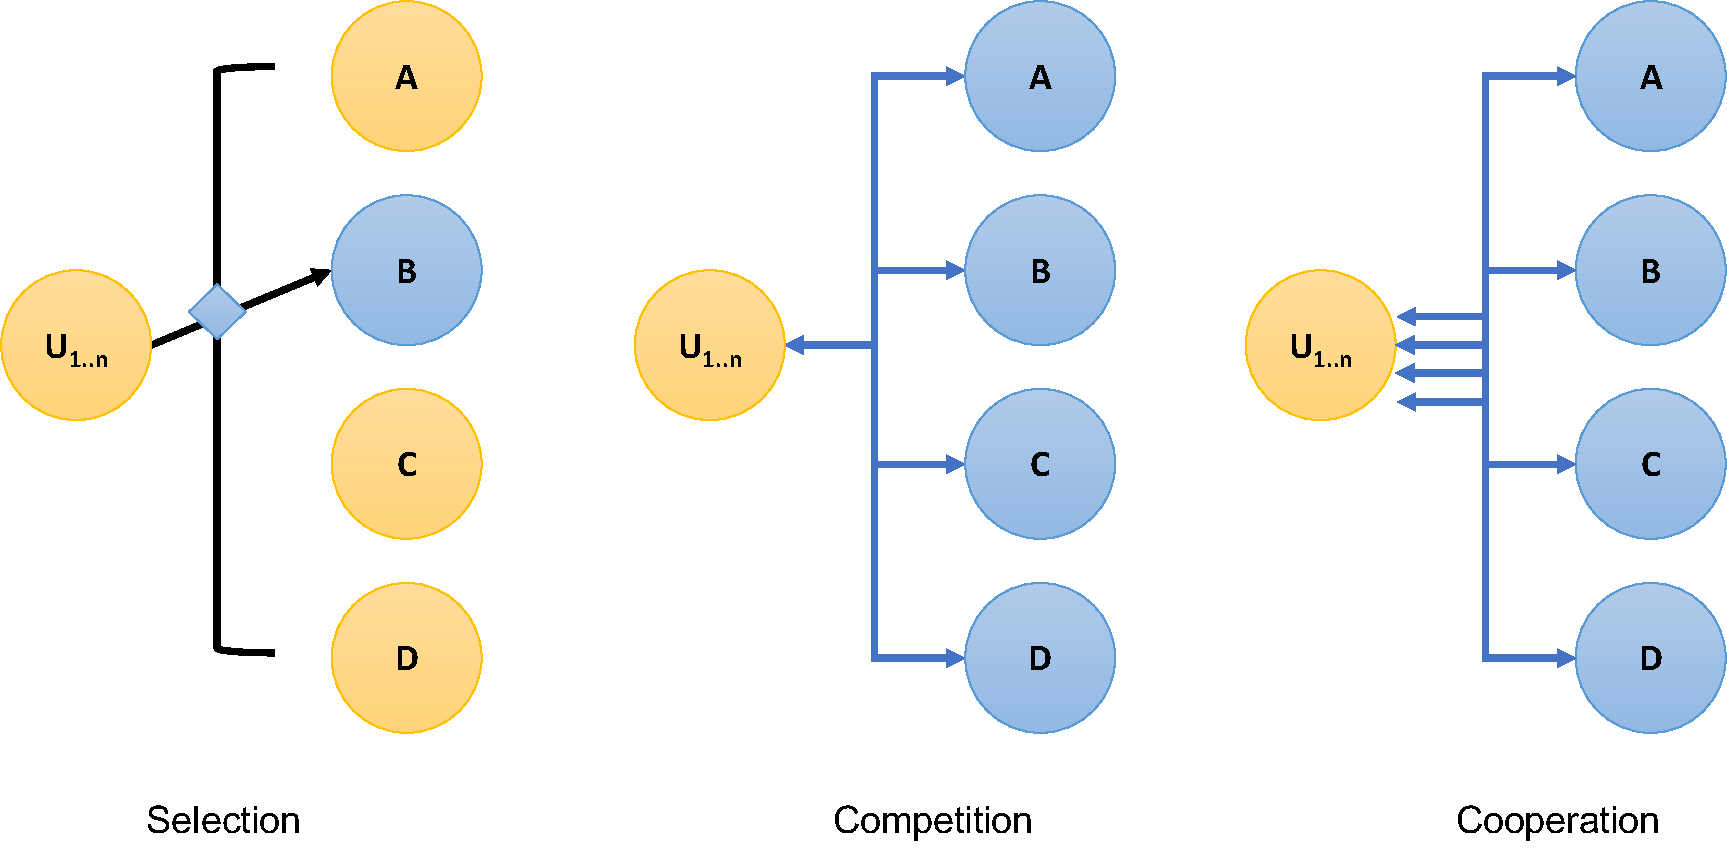
\includegraphics[width=0.75\columnwidth]{images/processes-nist.pdf}
\label{fig:service-interaction}
\caption{Service Interaction.}
\end{figure}


\subsubsection{Workflow Compute Coordinator}

High-performance computing (HPC) is for decades a very important tool
for science. Scientific tasks can be leveraging the processing power
of a supercomputer so they can run at previously unobtainable high
speeds or utilize specialized hardware for acceleration that otherwise
are not available to the user. HPC can be used for analytic programs
that leverage machine learning applied to large data sets to, for
example, predict future values or to model current states. For such
high-complexity projects, there are often multiple complex programs
that may be running repeatedly in either competition or cooperation.
This may include resources in the same or different data centers. We
developed a hybrid multi-cloud analytics service framework was created
to manage heterogeneous and remote workflows, queues, and jobs.  It
can be used through an Python API, the command line, and a REST
service. It is supported on multiple operating systems like macOS,
Linux, and Windows 10 and 11.  The workflow is specified via an easy
to define YAML file.  Specifically, we have developed a library called
Cloudmesh Compute Coordinator (cloudmesh-cc) that adds workflow
features to control the execution of jobs on remote compute resources,
while at the same time leveraging capabilities provided by the local
compute environments to directly interface with graphical
visualizations better suited for the desktop. The goal is to provide
numerous workflows that in cooperation enhances the experience of the
analytics tasks. This includes a REST service and command line tools
to interact with it.


\begin{figure}[htb]
\centering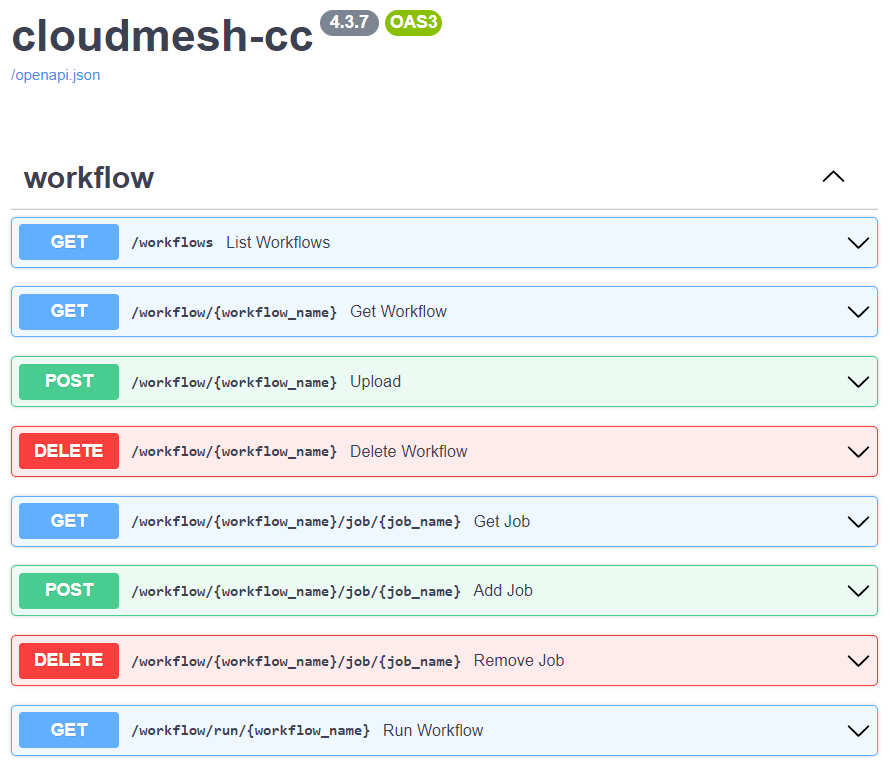
\includegraphics[width=0.7\columnwidth]{images/fastapi-service.png}
\caption{Fast API Workflow Service.}
% better resolution
\label{fig:fastapi-cc}
\end{figure}

\begin{figure}[htb]
    \centering
    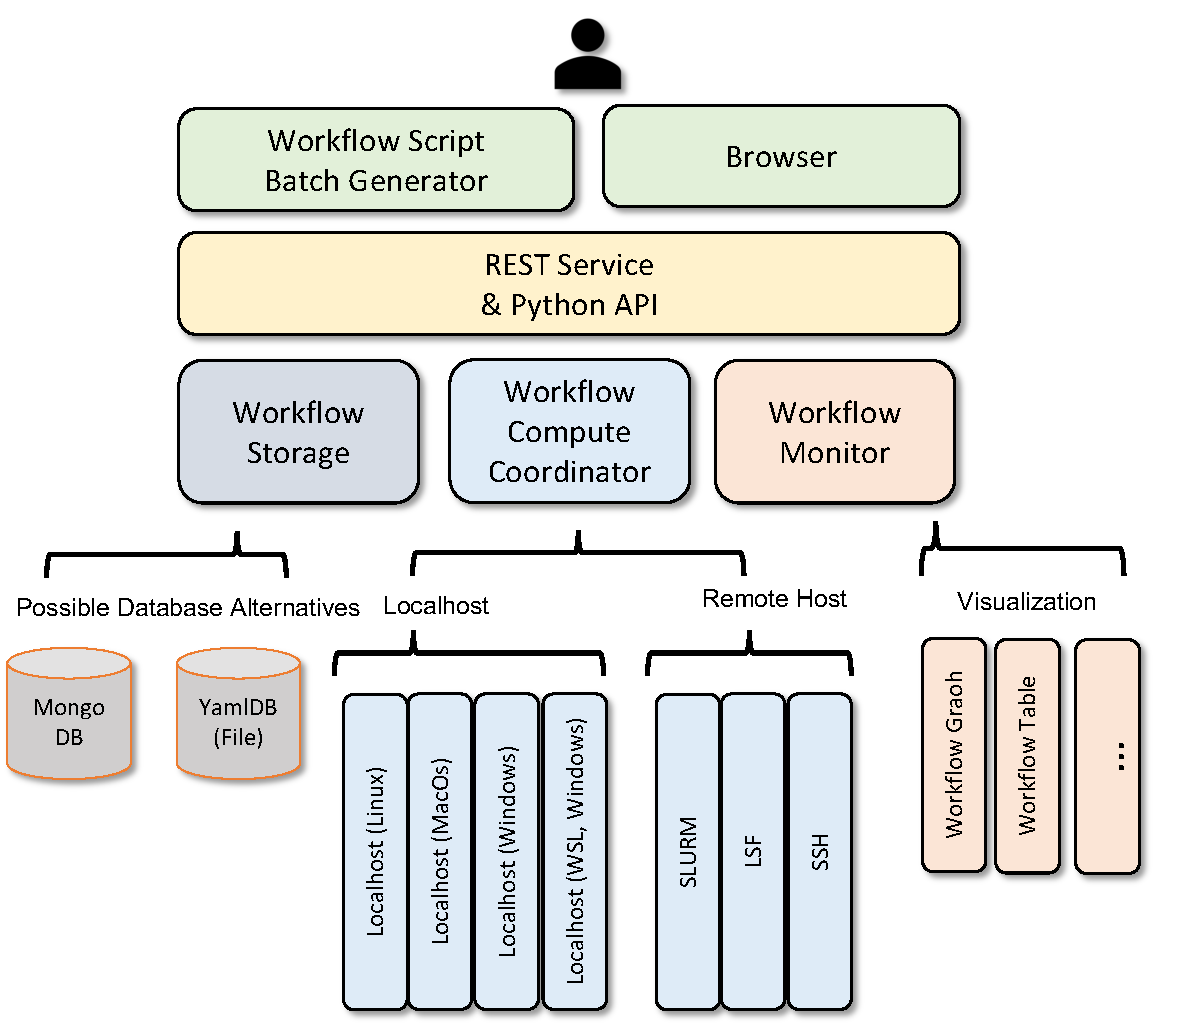
\includegraphics[width=0.50\columnwidth]{images/cloudmesh-cc-new.pdf}
    \caption{Architecture Workflow Service.}
    \label{fig:cc-2}
\end{figure}

\begin{figure}[htb]
    \centering
    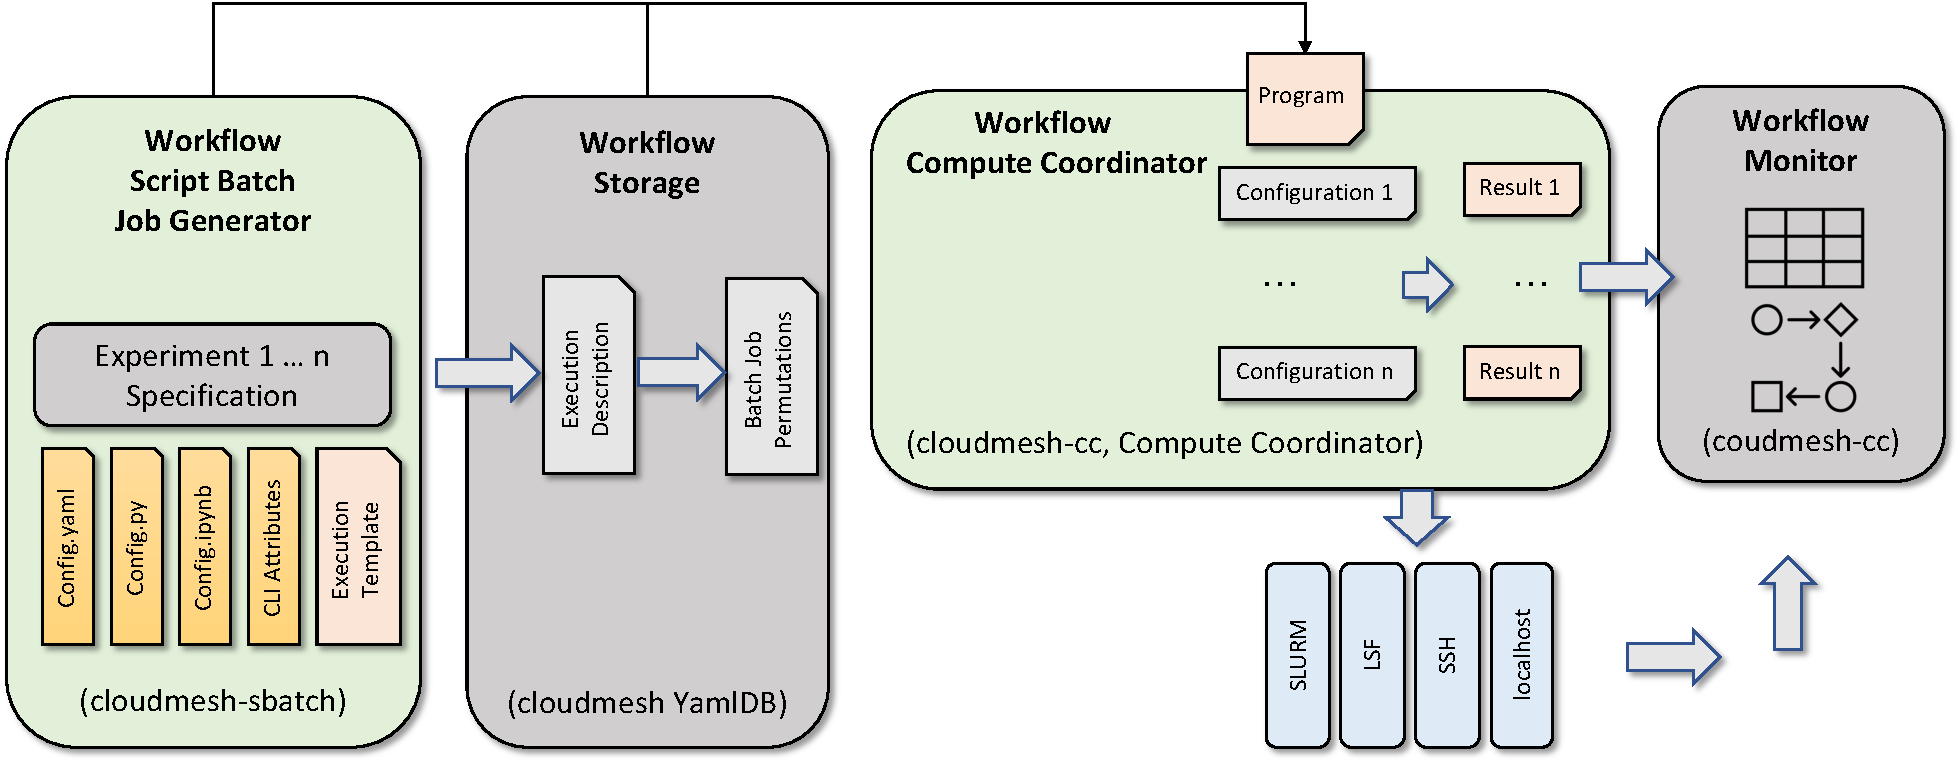
\includegraphics[width=0.70\columnwidth]{images/cloudmesh-sbatch-new.pdf}
    \caption{Workflow Script Batch Generator.}
    \label{fig:cm-sbatch}
\end{figure}



\begin{figure}[htb]
    \centering
    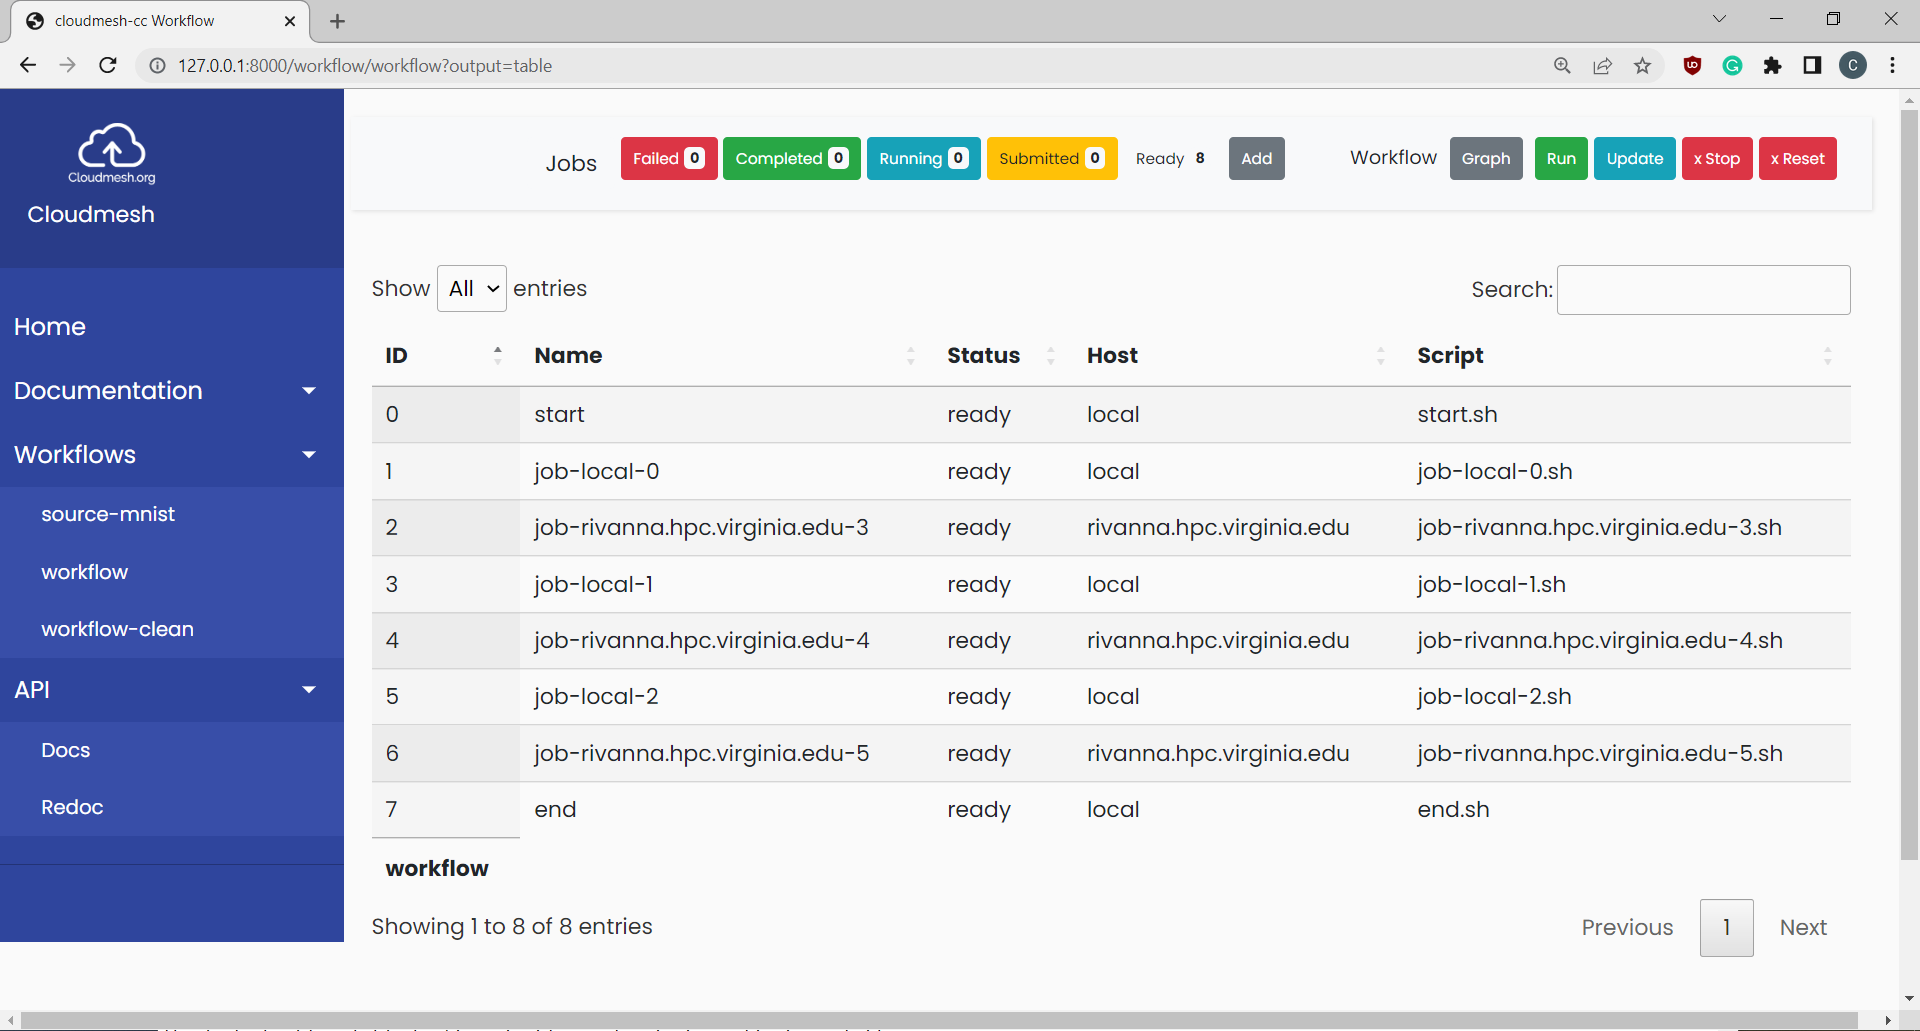
\includegraphics[width=0.70\columnwidth]{images/cc-1.png}
    \caption{Workflow user interface. }
    \label{fig:cc-3}
\end{figure}


We have tested the framework while running various MNIST application
examples, including include Multilayer Perceptron, LSTM (Long
short-term memory), Auto-Encoder, Convolutional, and Recurrent Neural
Networks, Distributed Training, and PyTorch training.  A much lager
application using earthquake prediction has also been used.

Figure \ref{fig:fastapi-cc} shows the REST specification and
\ref{fig:cc-2} shows the architecture.

% \subsubsection{Federated Analytics Service Catalogue}
% \subsubsection{Catalogue Attributes}
% \subsubsection{Federated analytics service Registries}
% \subsubsection{Registry Attributes}

% \subsection{Resource Accessibility}
% \subsubsection{Resource Management}
% \subsubsection{Security}




% three axis graph: system, software, science

\section{Nomenclature}

\subsection{Resource Identification Initiative}

{\bf Organization:} \verb|RRID:SCR_011743|

\section*{Conflict of Interest Statement}

The authors declare that the research was conducted in the absence of
any commercial or financial relationships that could be construed as a
potential conflict of interest.

\section*{Author Contributions}

{\em GvL} is the lead author and main contributor to this paper. He
has modified and augmented the earthquake paper to include the ability
to execute hyperparameters. {\em JPF} is a student that has
contributed to various aspects of the workflow component of the paper
and to a number of executions and evaluations of experiment runs. {\em
  RK} was a student and has helped together with {\em GVL} in the
implementation of cloudmesh-sbatch and the porting of the effort to
the UVA machine.  {\em GCF} is the author of the earthquake code and
facilitates the interactions with the MLCommons Science Working group
as a group leader of that effort.

\section*{Funding}

Work was in part funded by the NSF CyberTraining: CIC:
CyberTraining for Students and Technologies from Generation Z with the
award numbers 1829704 and 2200409 and NIST 60NANB21D151T. 
The work was also funded by the \TODO{Department of Energy under the
  grant ???.}
colleagues, institutions, or agencies that aided the efforts of the
authors.

\section*{Acknowledgments}

We like to thank Thomas Butler and Jake Kolessar for their
contributions during the capstone project while focusing on executing
initial runs of the code, and experimenting with modifications to the
code including logging. Please note that since this team finished
their work, significant improvements have been made by the authors of
this paper.

\section*{Data Availability Statement}

The code is all in public domain and available at GitHub at the following locations

\begin{itemize}

\item {\bf cloudmesh-cc} -- Is a code to control workflows to be executed on
  remote computing
  resources. \url{https://github.com/cloudmesh/cloudmesh-cc}

\item {\bf cloudmesh-sbatch} -- Is a code to generate batch scripts for
  hyperparameter studies high performance computers so they can be
  executed on different suppercomputers by multiple
  accounts. \url{https://github.com/cloudmesh/cloudmesh-sbatch}

\item {\bf cloudmesh} -- Cloudmesh is a large collection of repositories for
  accessing cloud and HPC
  resources. \url{https://github.com/orgs/cloudmesh/repositories}

\item {\bf mlcommons eartchquake production code} -- The MLCommons Sceience
  Working group is described at
  \url{https://mlcommons.org/en/groups/research-science/}. This page
  contains the links to the production level earthquake code.

\item {\bf mlcommons eartchquake development code} -- The development version of
  the code is available in this reporitory. It also contains many of
  the analysis scrripts that are not pare of the production code
  hosted by MLCommons \url{https://github.com/laszewsk/mlcommons}.
  
\end{itemize}


% \bibliographystyle{Frontiers-Harvard}

\bibliographystyle{Frontiers-Vancouver} % Many Frontiers journals
% use the numbered referencing system, to find the style and resources
% for the journal you are submitting to:
% https://zendesk.frontiersin.org/hc/en-us/articles/360017860337-Frontiers-Reference-Styles-by-Journal

\bibliography{vonLaszewski-references}


\section*{Figure captions}

%%% max 15 figures abd table, subfig is one figure

%%%  NB logo1.eps is required in the path in order to correctly compile front page header %%%



\begin{figure}[htb]

  \begin{center}

     \begin{minipage}[b]{0.45\textwidth}
       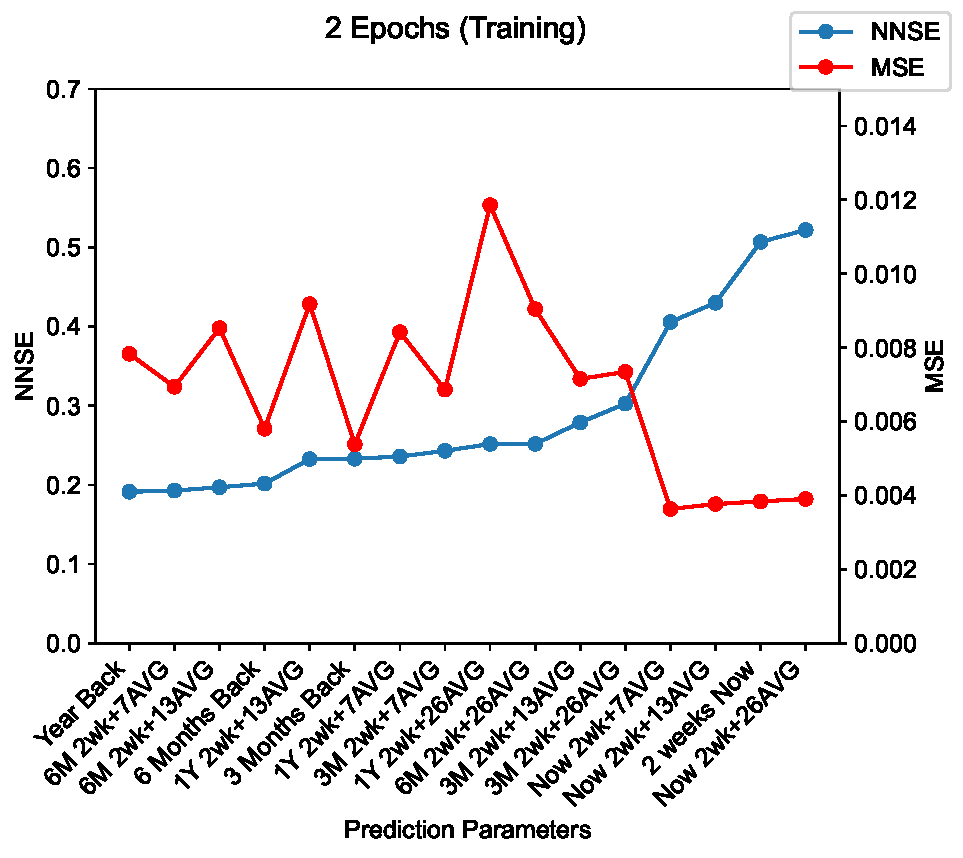
\includegraphics[width=1.0\linewidth]{images/2_training-MSE-and-NNSE.pdf}
        {\bf (A)} MSE and NNSE - 2 epochs training.
    \end{minipage}
     \ \
     \begin{minipage}[b]{0.45\textwidth}
        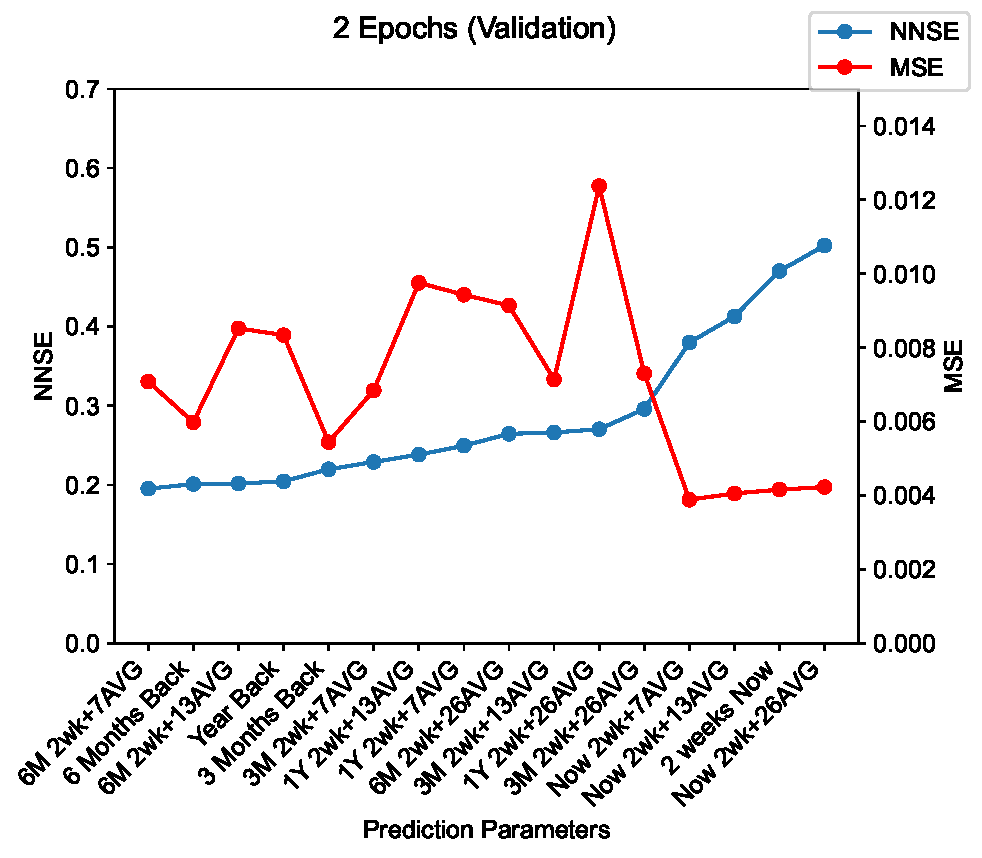
\includegraphics[width=1.0\linewidth]{images/2_validation-MSE-and-NNSE.pdf}
        {\bf (B)}  MSE and NNSE - 2 epochs validation.
     \end{minipage}

     \begin{minipage}[b]{0.45\textwidth}
        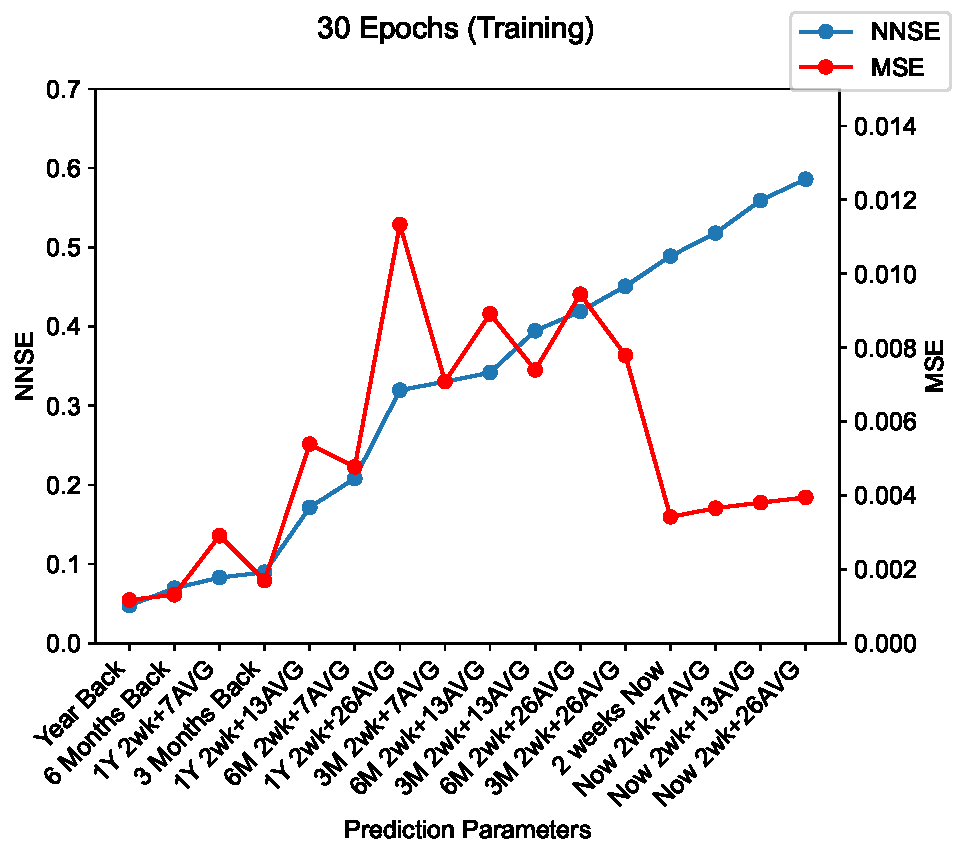
\includegraphics[width=1.0\linewidth]{images/30_training-MSE-and-NNSE.pdf}
        {\bf (C)} MSE and NNSE - 30 epochs training.
     \end{minipage}
     \ \
     \begin{minipage}[b]{0.45\textwidth}
        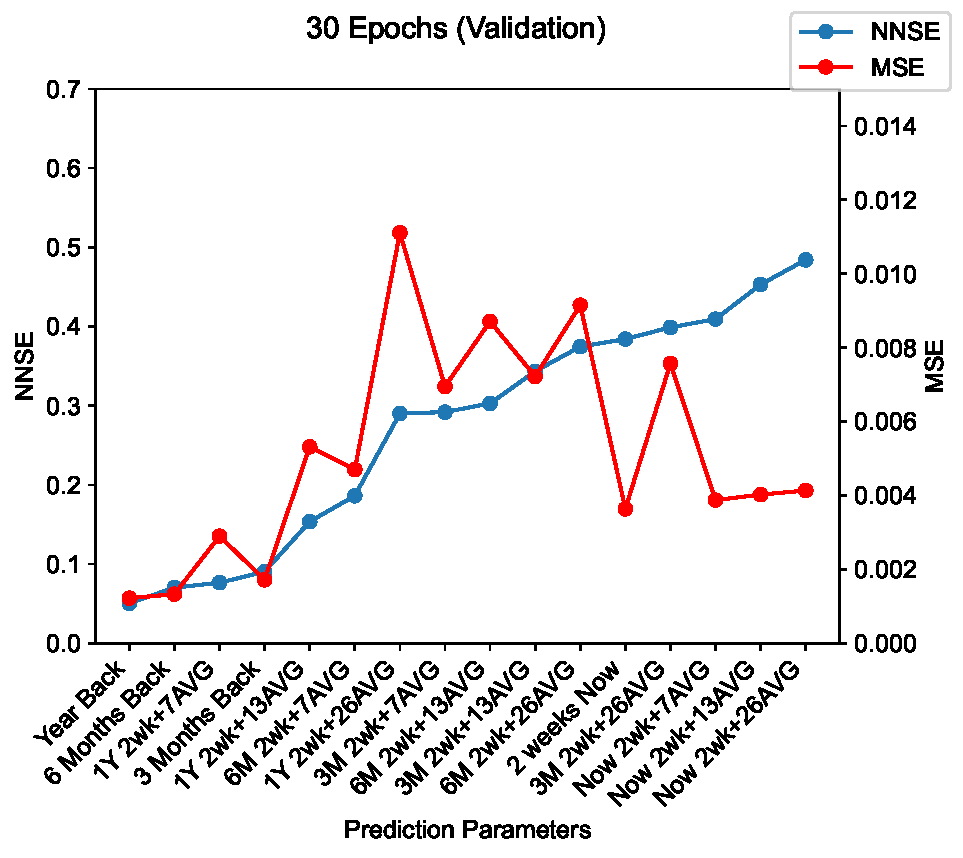
\includegraphics[width=1.0\linewidth]{images/30_validation-MSE-and-NNSE.pdf}
        {\bf (D)} MSE and NNSE - 30 epochs validation.
     \end{minipage}

     \begin{minipage}[b]{0.45\textwidth}
        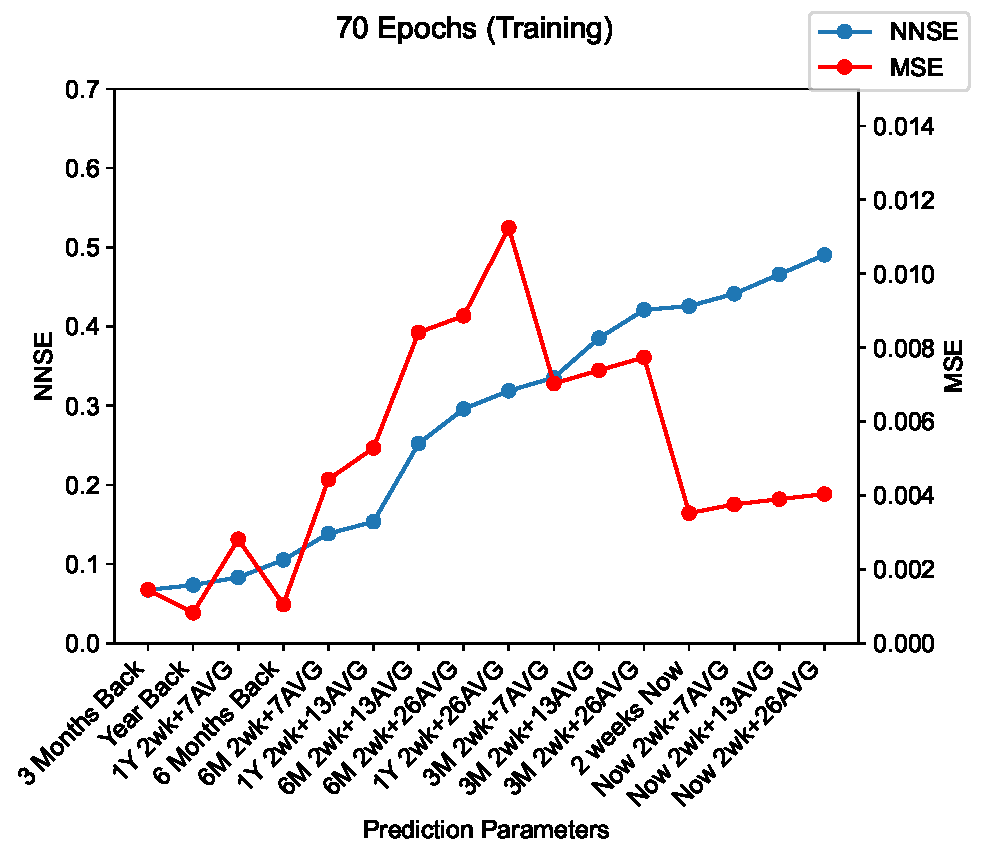
\includegraphics[width=1.0\linewidth]{images/70_training-MSE-and-NNSE.pdf}
        {\bf (E)} MSE and NNSE - 70 epochs training.
     \end{minipage}
     \ \
     \begin{minipage}[b]{0.45\textwidth}
        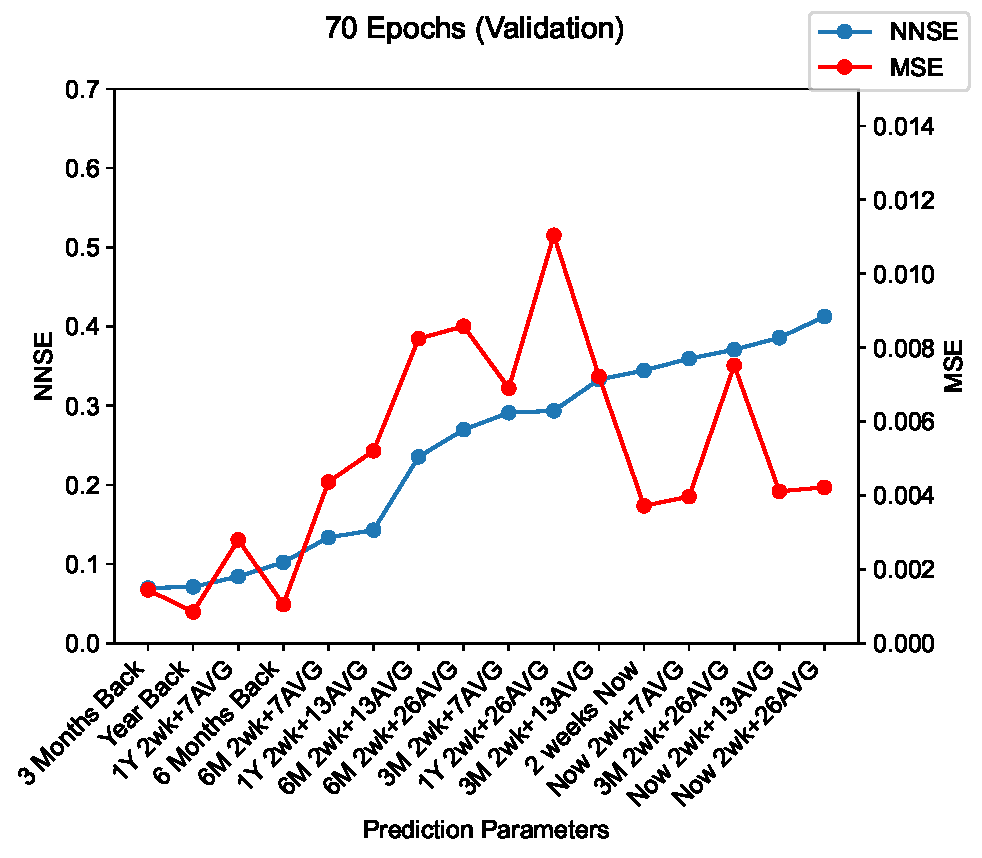
\includegraphics[width=1.0\linewidth]{images/70_validation-MSE-and-NNSE.pdf}
        {\bf (F)}  MSE and NNSE - 70 epochs validation.
     \end{minipage}
\end{center}
     
     \caption{NNSE and MSE values for training and validation for epochs 2 (A, B), 30 (C, D), 70 (E, F).}
     \label{fig:six graphs}
\end{figure}

%we have finalized the EQ code but want to make absolutely sure that we
%look at the correct values for the scientific comparison.
%
%This also requires a small sentence to each variable. Could we have a
%small meeting and I take then some notes on what these values are
%tomorrow. I will then add the explanations to the MLCommons EQ benchmark
%policy document.
%
%I just want to make sure I understand over which domain we average and
%sum up.
%
%Also if we were to just do one value (just in case they ask, I think we
%would use the summed up total right. However I think it is better to
%keep all of them.)
%
%Also I forgot what the +26 refers to
%
%I think soething like this is almost correct, but we need to +26
%explanation and get verification from you.
%
%The Magnification based on a years worth of back data, while looking two
%weeks ahead + 26 what?

\begin{table}[htb]

  \caption{Training and validation with time based hyperparameters
    sorted by NNSE accuracy. The table includes the best two two
    values highlighted in the training and validation results to
    showcase the the the accuracy of the validation. In the validation
    we see that the best value for training is in rank four for the
    validation. The number of Epochs for this experiment is 2.
    26 is half of 52 and so 26 2-week intervals is a year.}
  \label{tab:training-2}

  \renewcommand{\arraystretch}{1.2}
\begin{center}
\begin{tabular}{|r|rl||rl|}
  \hline
{\bf Rank} & \multicolumn{2}{c||}{\bfseries Training} & \multicolumn{2}{c|}{\bfseries Validation}  \\
     &   {\bf NNSE} & {\bf Hyperparameters} & {\bf NNSE} & {\bf Hyperparameters} \\
\hline
1 & \color{red} 0.191300 & \color{red} Year Back & \color{blue} 0.195200 & \color{blue} 6M 2wk+7AVG \\
2 & 0.192700 & \color{blue} 6M 2wk+7AVG & \color{teal} 0.201000 & \color{teal} 6 Months Back \\
3 & 0.197000 & 6M 2wk+13AVG & 0.201600 & 6M 2wk+13AVG \\
4 & \color{teal} 0.201600 & \color{teal} 6 Months Back & \color{red} 0.204500 & \color{red} Year Back \\
5 & 0.232600 & 1Y 2wk+13AVG & 0.219700 & 3 Months Back \\
6 & 0.233000 & 3 Months Back & 0.228900 & 3M 2wk+7AVG \\
7 & 0.235800 & 1Y 2wk+7AVG & 0.238200 & 1Y 2wk+13AVG \\
8 & 0.243000 & 3M 2wk+7AVG & 0.249500 & 1Y 2wk+7AVG \\
9 & 0.251600 & 1Y 2wk+26AVG & 0.264400 & 6M 2wk+26AVG \\
10 & 0.251700 & 6M 2wk+26AVG & 0.266200 & 3M 2wk+13AVG \\
11 & 0.278800 & 3M 2wk+13AVG & 0.270300 & 1Y 2wk+26AVG \\
12 & 0.302500 & 3M 2wk+26AVG & 0.295800 & 3M 2wk+26AVG \\
13 & 0.405600 & Now 2wk+7AVG & 0.379700 & Now 2wk+7AVG \\
14 & 0.429900 & Now 2wk+13AVG & 0.412700 & Now 2wk+13AVG \\
15 & 0.506800 & 2 weeks Now & 0.470100 & 2 weeks Now \\
16 & 0.521800 & Now 2wk+26AVG & 0.502300 & Now 2wk+26AVG \\
\hline
\end{tabular}
\end{center}

\end{table}

\begin{table}[htb]

  \caption{Training and validation with time based hyperparameters
    sorted by NNSE accuracy. The table includes the best two two
    values highlighted in the training and validation results to
    showcase the the the accuracy of the validation. In the validation
    we see that the best value for training is in rank four for the
    validation. The number of Epochs for this experiment is 30.
  }
  \label{tab:training-30}

  \renewcommand{\arraystretch}{1.2}
\begin{center}
\begin{tabular}{|r|rl||rl|}
\hline
{\bf Rank} &
\multicolumn{2}{c||}{\bfseries Training} &
\multicolumn{2}{c|}{\bfseries Validation} \\
     {\bf NNSE} &
     {\bf Hyperparameters} &
     {\bf NNSE} &
     {\bf Hyperparameters} \\
\hline
 1 & \color{red} 0.047600 & \color{red} Year Back & \color{red} 0.050500 & \color{red} Year Back \\
 2 & \color{blue} 0.069500 & \color{blue} 6 Months Back & \color{blue} 0.070300 & \color{blue} 6 Months Back \\
 3 & 0.082900 & 1Y 2wk+7AVG & 0.076500 & 1Y 2wk+7AVG \\
 4 & 0.089700 & 3 Months Back & 0.090400 & 3 Months Back \\
 5 & 0.171600 & 1Y 2wk+13AVG & 0.153600 & 1Y 2wk+13AVG \\
 6 & 0.208100 & 6M 2wk+7AVG & 0.186200 & 6M 2wk+7AVG \\
 7 & 0.319600 & 1Y 2wk+26AVG & 0.290100 & 1Y 2wk+26AVG \\
 8 & 0.330300 & 3M 2wk+7AVG & 0.291900 & 3M 2wk+7AVG \\
 9 & 0.341800 & 6M 2wk+13AVG & 0.302800 & 6M 2wk+13AVG \\
10 & 0.394600 & 3M 2wk+13AVG & 0.343400 & 3M 2wk+13AVG \\
11 & 0.418900 & 6M 2wk+26AVG & 0.374500 & 6M 2wk+26AVG \\
12 & 0.450800 & 3M 2wk+26AVG & 0.384100 & 2 weeks Now \\
13 & 0.488800 & 2 weeks Now & 0.398900 & 3M 2wk+26AVG \\
14 & 0.517900 & Now 2wk+7AVG & 0.409300 & Now 2wk+7AVG \\
15 & 0.559200 & Now 2wk+13AVG & 0.453000 & Now 2wk+13AVG \\
16 & 0.586000 & Now 2wk+26AVG & 0.484100 & Now 2wk+26AVG \\
\hline
\end{tabular}

\end{center}
\end{table}


\begin{table}[htb]

  \caption{Training and validation with time based hyperparameters
    sorted by NNSE accuracy. The table includes the best two two
    values highlighted in the training and validation results to
    showcase the the the accuracy of the validation. In the validation
    we see that the best value for training is in rank four for the
    validation. The number of Epochs for this experiment is 70.}
  \label{tab:training-70}

  \renewcommand{\arraystretch}{1.2}
\begin{center}
\begin{tabular}{|r|rl||rl|}
  \hline
{\bf Rank} & \multicolumn{2}{c||}{\bfseries Training} & \multicolumn{2}{c|}{\bfseries Validation} \\
     &   {\bf NNSE} & {\bf Hyperparameters} & {\bf NNSE} & {\bf Hyperparameters} \\
              \hline
 1 & \color{red} 0.067400 & \color{red} 3 Months Back & \color{red}0.069800 & \color{red} 3 Months Back \\
 2 & \color{blue} 0.073500 & \color{blue} Year Back & \color{blue} 0.071200 & \color{blue} Year Back \\
 3 & 0.083100 & 1Y 2wk+7AVG & 0.084300 & 1Y 2wk+7AVG \\
 4 & 0.105300 & 6 Months Back & 0.102200 & 6 Months Back \\
 5 & 0.138400 & 6M 2wk+7AVG & 0.133700 & 6M 2wk+7AVG \\
 6 & 0.153500 & 1Y 2wk+13AVG & 0.142800 & 1Y 2wk+13AVG \\
 7 & 0.252100 & 6M 2wk+13AVG & 0.235400 & 6M 2wk+13AVG \\
 8 & 0.295900 & 6M 2wk+26AVG & 0.269700 & 6M 2wk+26AVG \\
 9 & 0.318800 & 1Y 2wk+26AVG & 0.291100 & 3M 2wk+7AVG \\
10 & 0.335400 & 3M 2wk+7AVG & 0.293500 & 1Y 2wk+26AVG \\
11 & 0.385200 & 3M 2wk+13AVG & 0.333000 & 3M 2wk+13AVG \\
12 & 0.421000 & 3M 2wk+26AVG & 0.344500 & 2 weeks Now \\
13 & 0.425700 & 2 weeks Now & 0.359400 & Now 2wk+7AVG \\
14 & 0.441300 & Now 2wk+7AVG & 0.370700 & 3M 2wk+26AVG \\
15 & 0.465800 & Now 2wk+13AVG & 0.385800 & Now 2wk+13AVG \\
16 & 0.490400 & Now 2wk+26AVG & 0.412500 & Now 2wk+26AVG \\
\hline
\end{tabular}
\end{center}

\end{table}


\section{Energy}

\begin{figure}[htb]

  \begin{center}
     \begin{minipage}[t]{0.30\textwidth}
        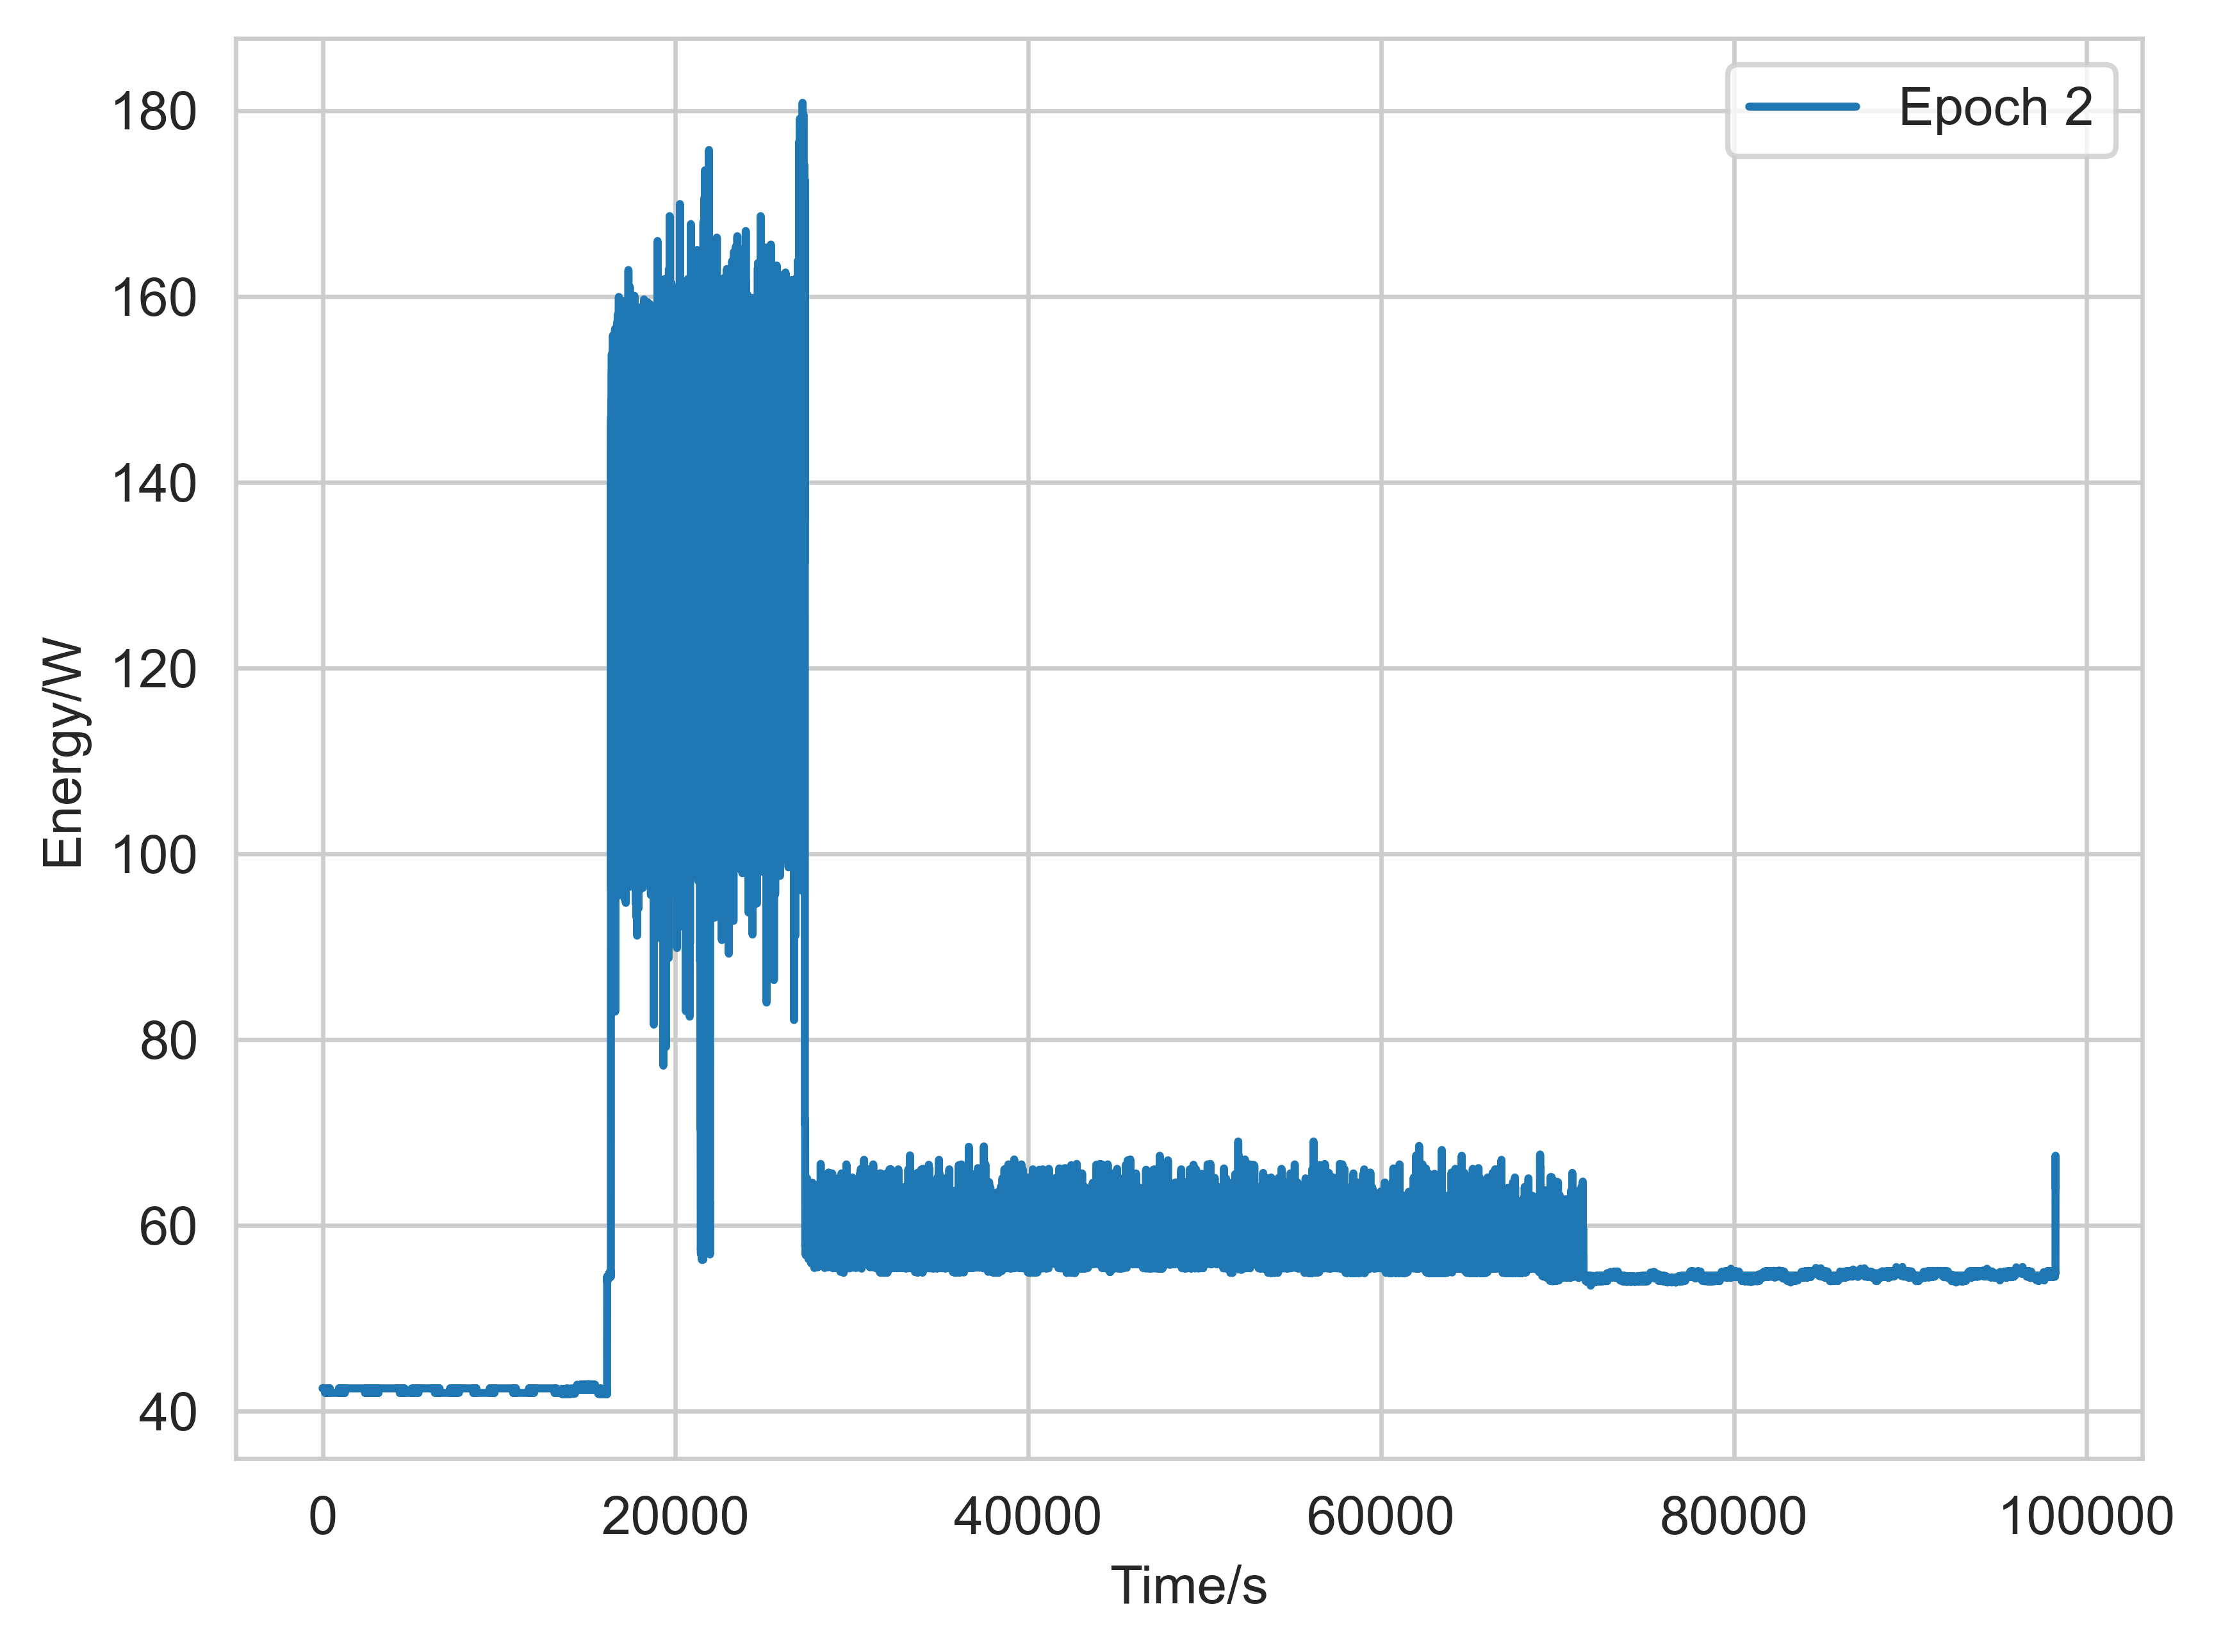
\includegraphics[width=1.0\linewidth]{images/card-name-v100-gpu-count-1-cpu-num-6-mem-32gb-repeat-1-tfttransformerepochs-2.png}
        {\bf (A)} Energy consumption for 2 epochs training and validation.
     \end{minipage}
     \ \
     \begin{minipage}[t]{0.30\textwidth}
        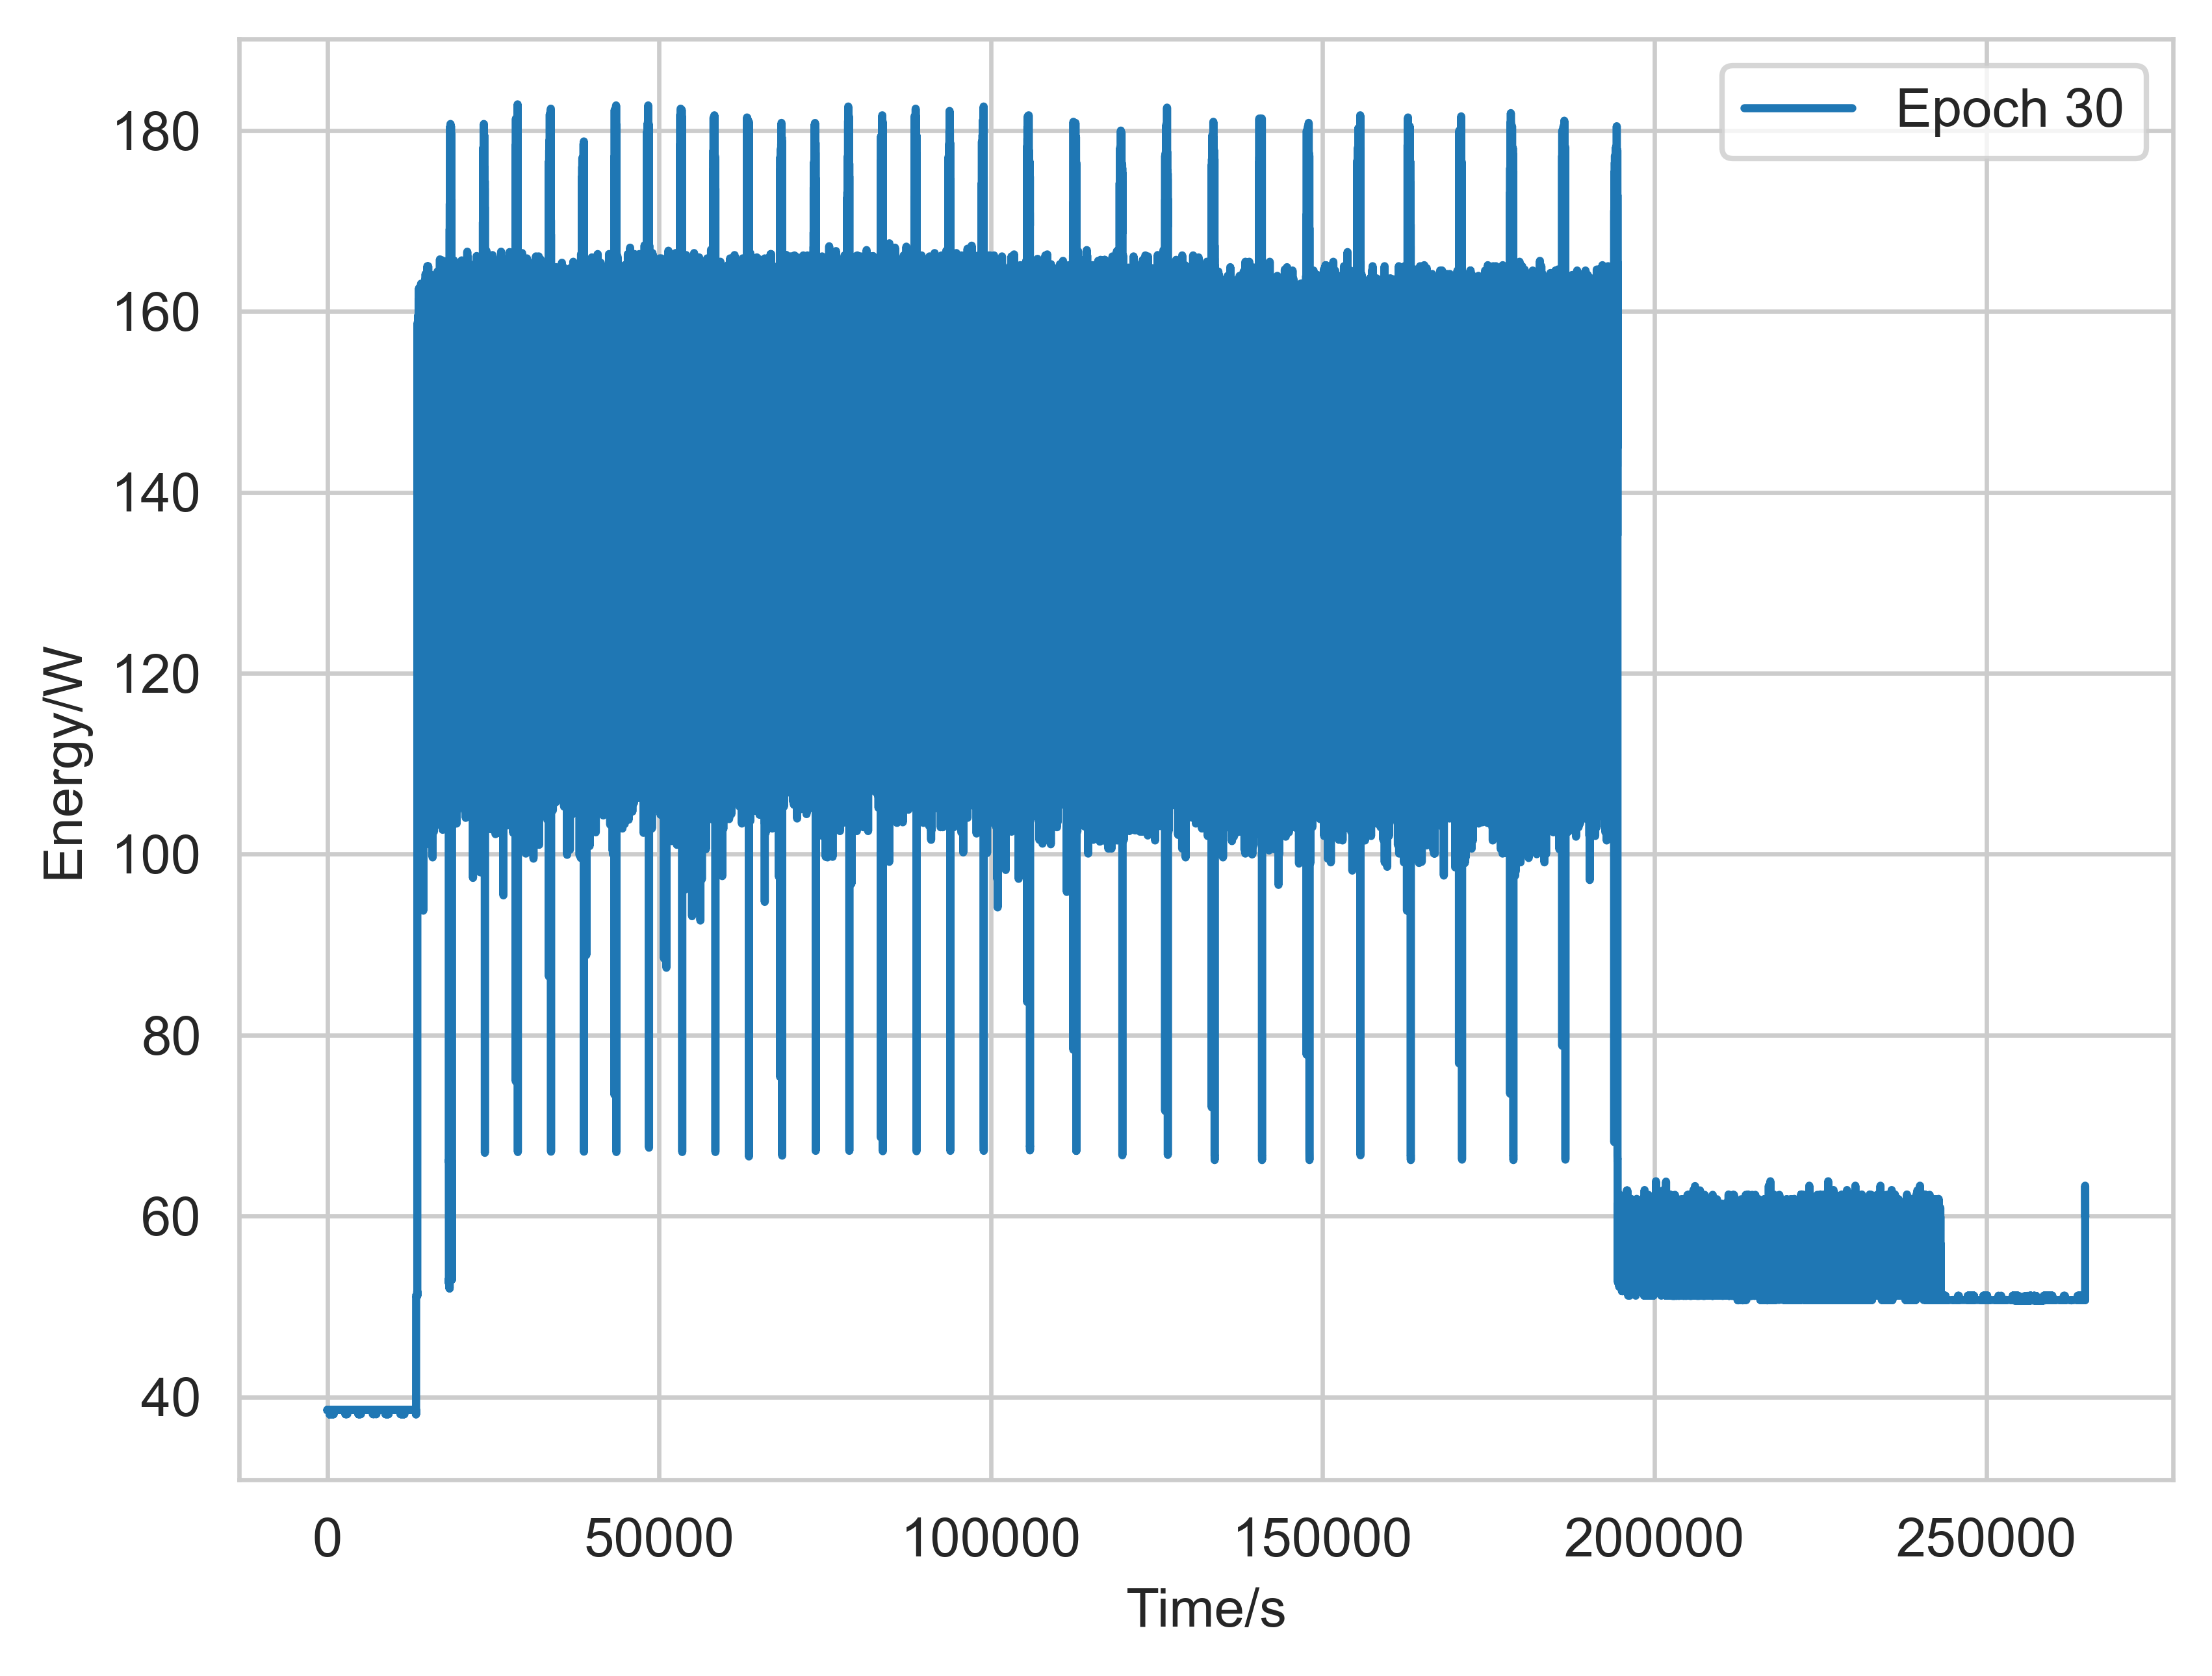
\includegraphics[width=1.0\linewidth]{images/card-name-v100-gpu-count-1-cpu-num-6-mem-32gb-repeat-1-tfttransformerepochs-30.png}
        {\bf (B)} Energy consumption for 30 epochs training and validation.
     \end{minipage}
     \ \
     \begin{minipage}[t]{0.30\textwidth}
        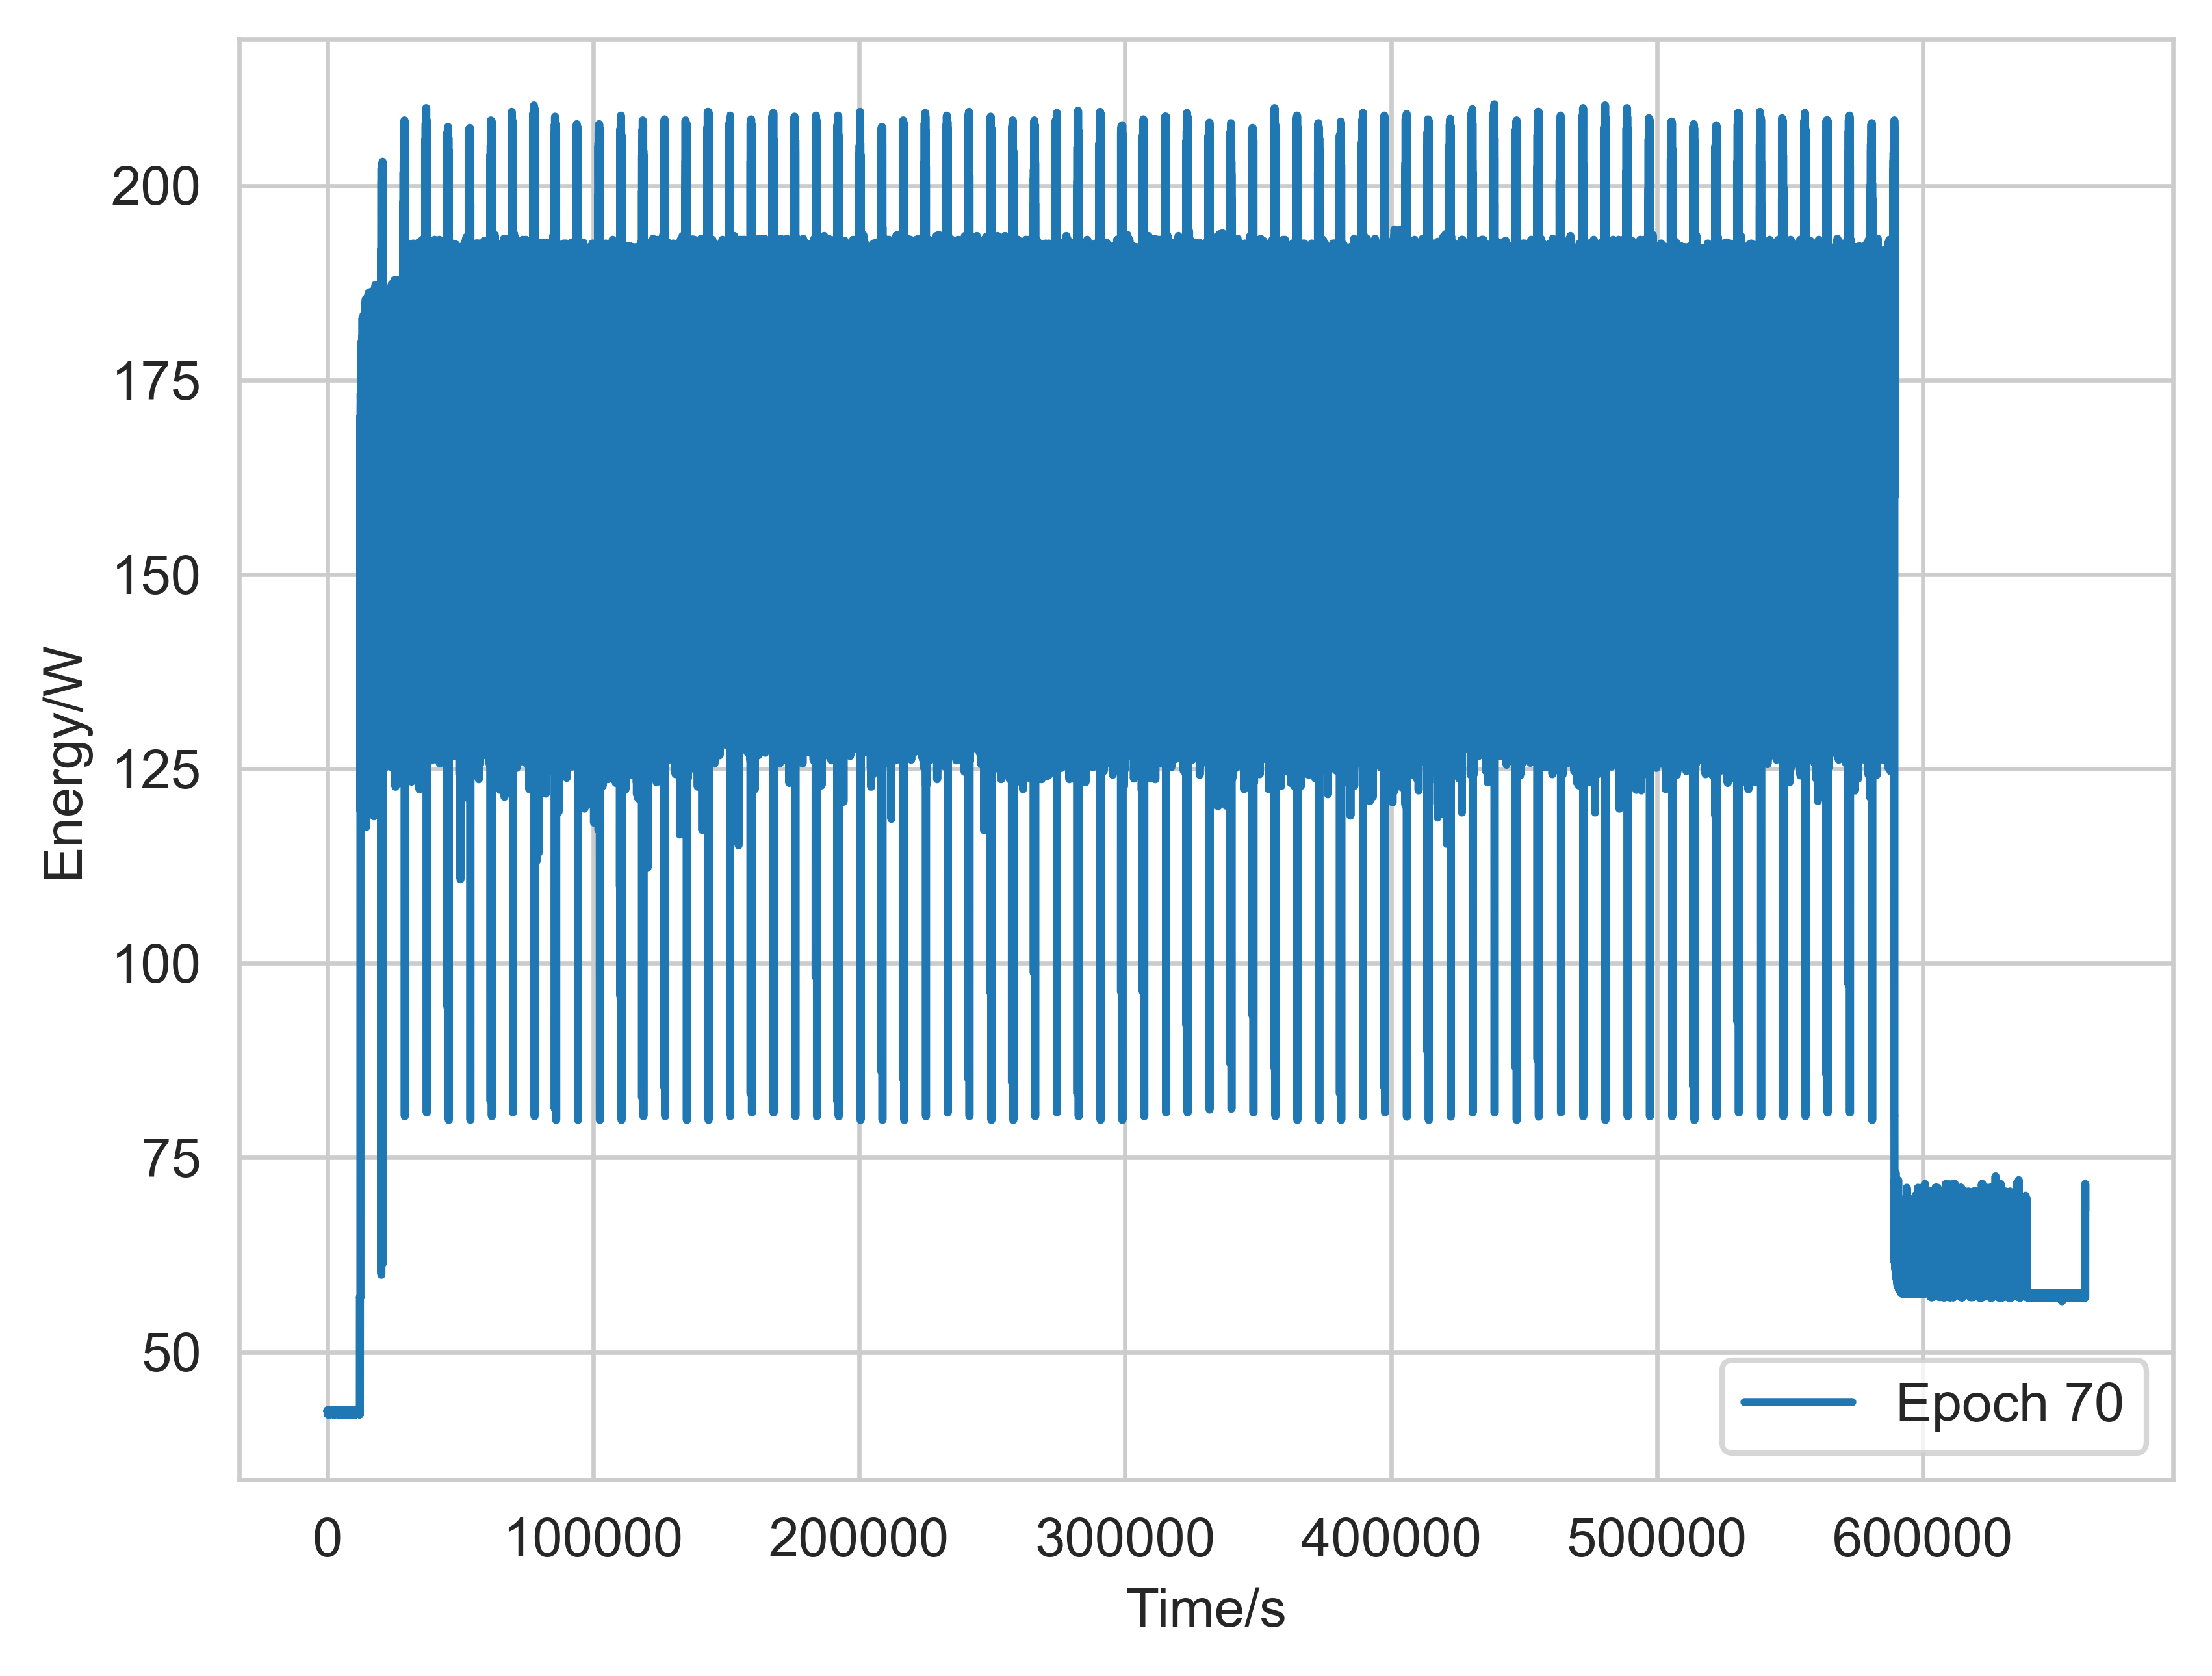
\includegraphics[width=1.0\linewidth]{images/card-name-v100-gpu-count-1-cpu-num-6-mem-32gb-repeat-1-tfttransformerepochs-70.png}
        {\bf (C)} Energy consumption for 70 epochs training and validation.
     \end{minipage}
  \end{center}

  \caption {Energy monitoring for 2, 30, and 70 epochs for training and validation.}
  \label{fig:energy}

\end{figure}

\begin{figure}[htb]

  \begin{center}
     \begin{minipage}[t]{0.30\textwidth}
        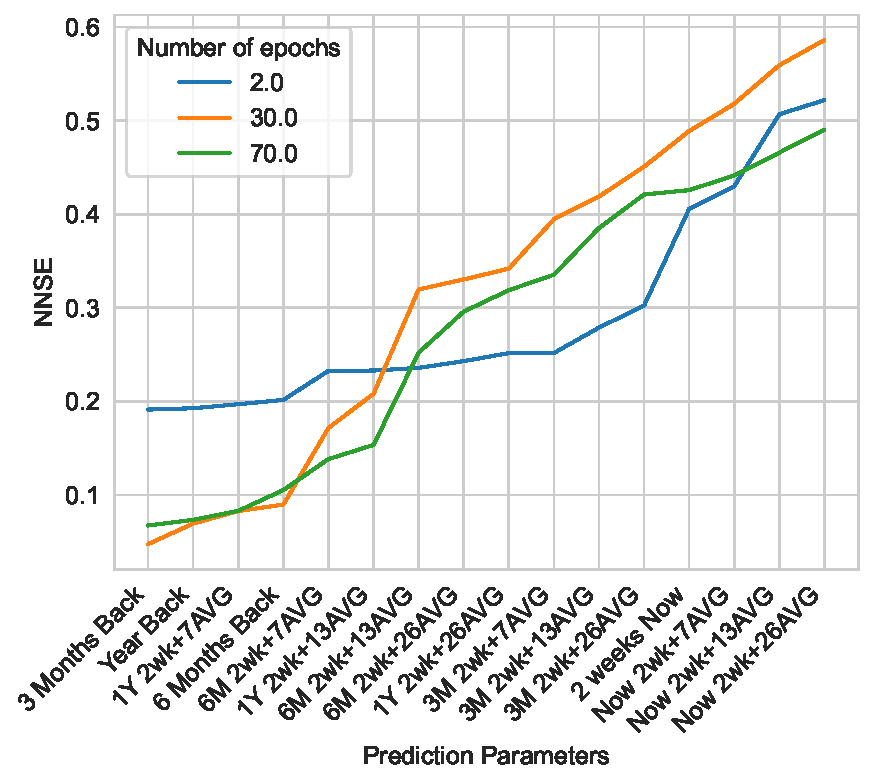
\includegraphics[width=1.0\linewidth]{images/NNSE-all-epochs-training}
        {\bf (A)} NNSE for training.
     \end{minipage}
  \end{center}
  \ \
  \begin{center}
     \begin{minipage}[t]{0.30\textwidth}
        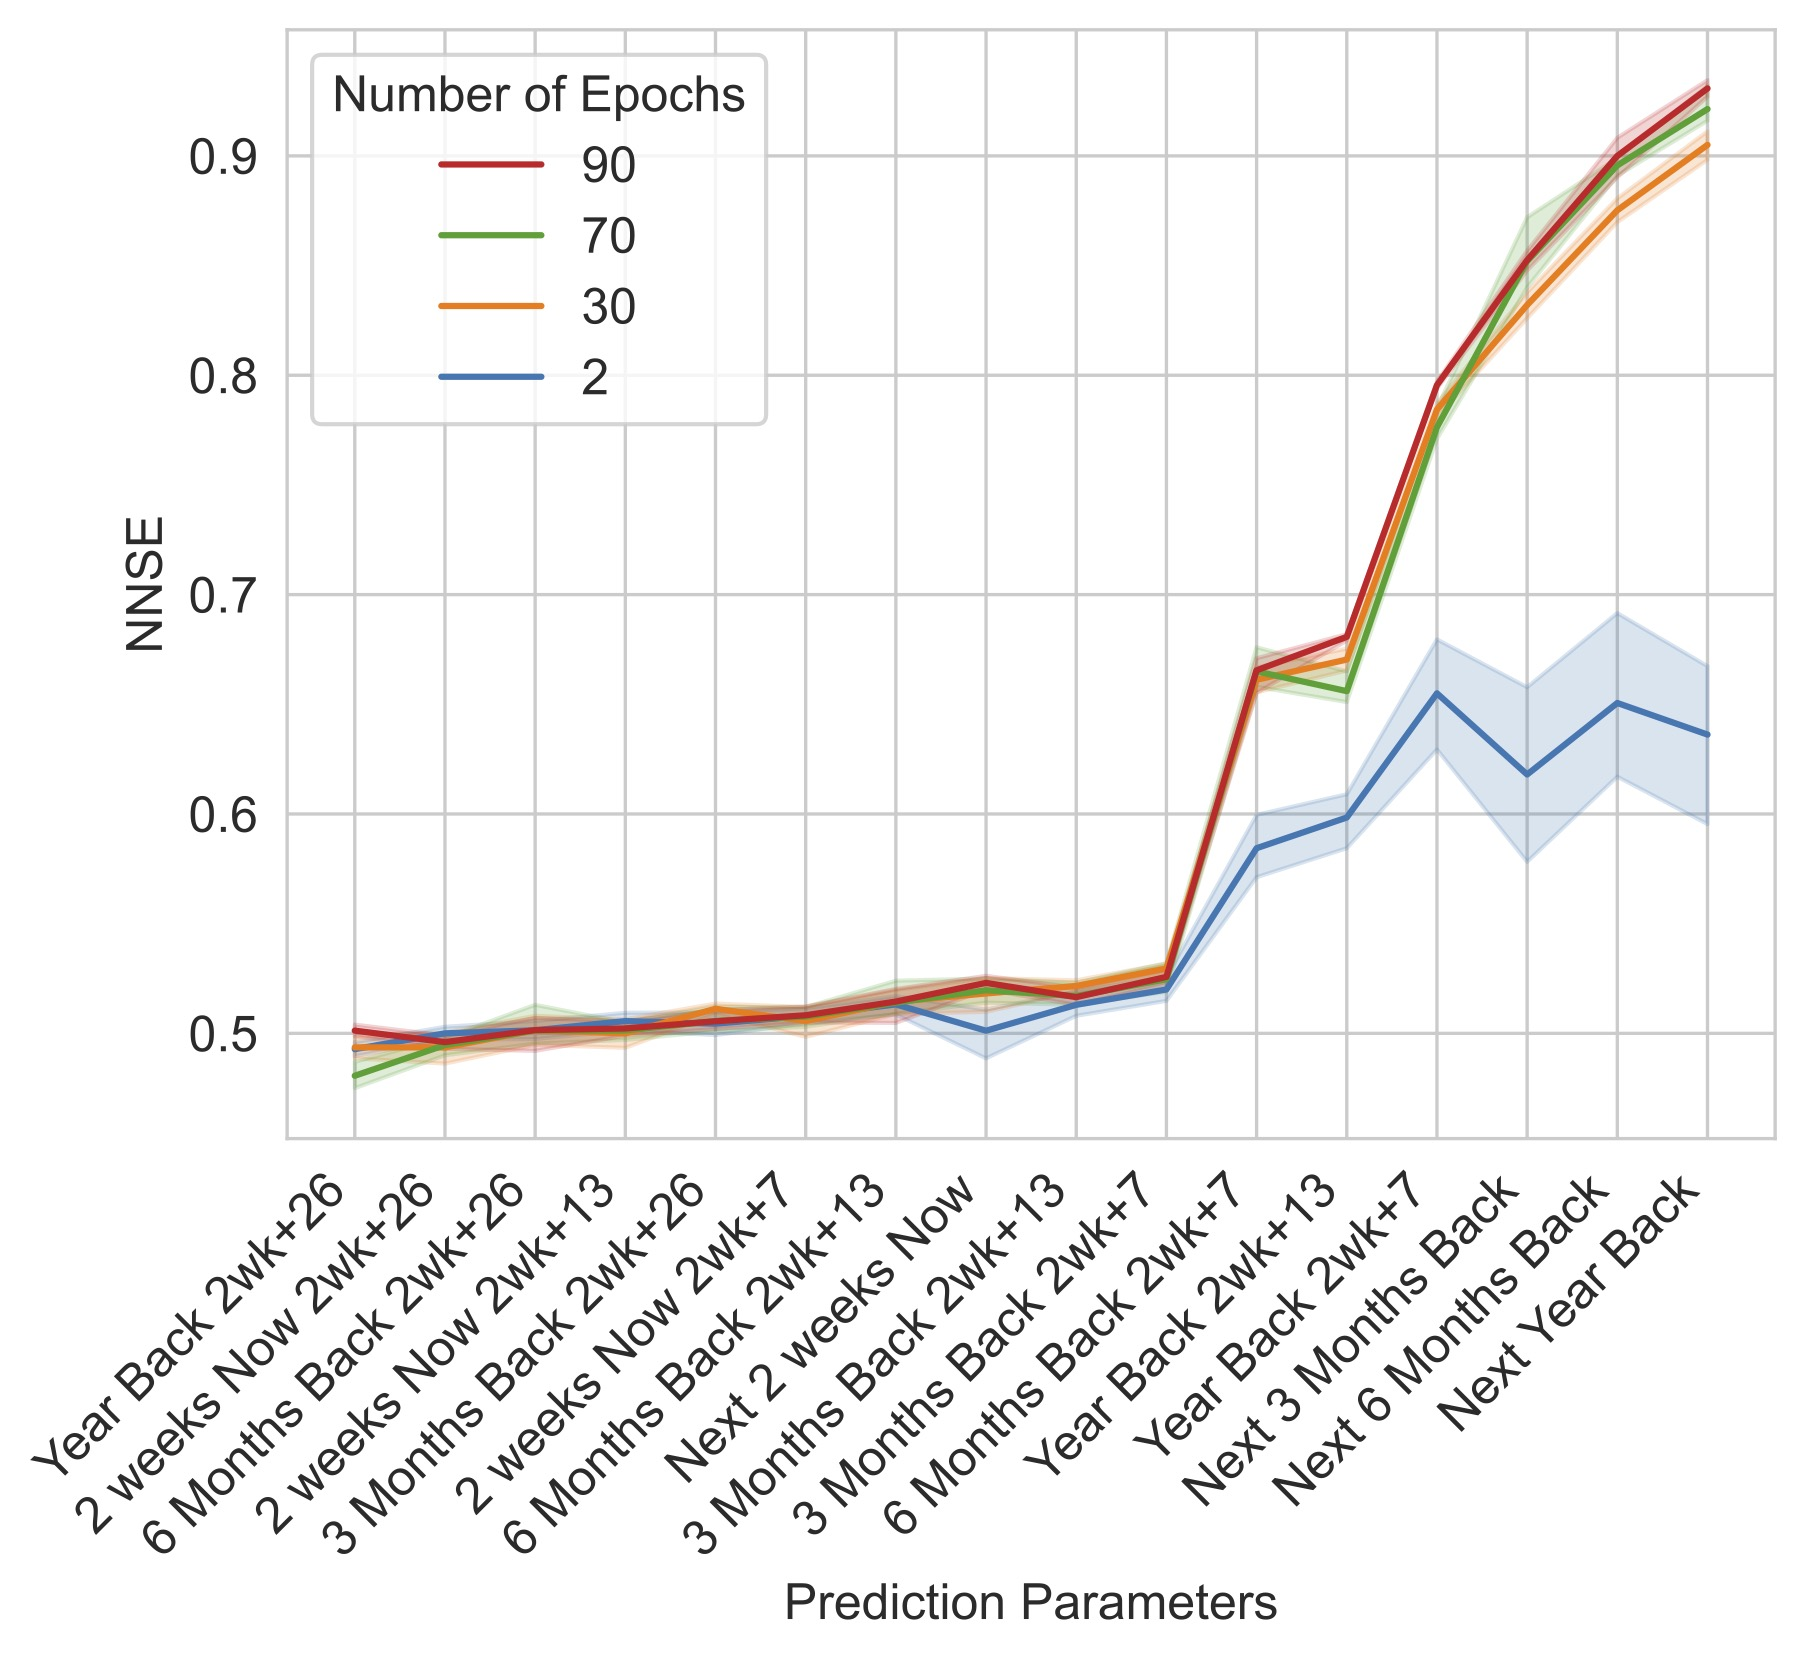
\includegraphics[width=1.0\linewidth]{images/NNSE-all-epochs-validation}
        {\bf (B)} NNSE for validation.
     \end{minipage}
  \end{center}

  \caption {NNSE comparison}
  \label{fig:NNSE-comparison}

\end{figure}

\end{document}
